\documentclass[11pt, a4paper]{report}
\usepackage[a4paper, width=150mm, top=35mm, bottom=35mm]{geometry}
\usepackage[utf8]{inputenc}
\usepackage{tikz}
\usepackage{amsthm}
\usetikzlibrary{calc}
\usepackage{graphicx}
\usepackage{float}
\usepackage{enumerate}
\usepackage{longtable}
\usepackage{fancyhdr}
\usepackage{listings}
\usepackage{xcolor}
\usepackage{mathtools}
\usepackage{tabularx}
\usepackage{titlesec}
\usepackage[shortlabels]{enumitem}
\usepackage{amssymb}
\usepackage{multirow}
\renewcommand{\chaptername}{BAB}
\renewcommand{\figurename}{Gambar}
\renewcommand{\tablename}{Tabel}
\renewcommand{\contentsname}{DAFTAR ISI}
\renewcommand{\listtablename}{DAFTAR TABEL}
\renewcommand{\listfigurename}{DAFTAR GAMBAR}
\pagestyle{fancy}
\graphicspath{{images/}}
\titleformat{\chapter}[display]
{\normalfont\huge\bfseries\centering}{\chaptertitlename\ \thechapter}{20pt}{\Huge}
\begin{document}
\begin{titlepage}
\begin{center}
	
\begin{tikzpicture}[remember picture, overlay]
		\draw[line width = 1pt] ($(current page.north west) + (1in,-1in)$) rectangle ($(current page.south east) + (-1in,1in)$);
	\end{tikzpicture}
	
	\Large
	\textbf{SISTEM MARKETPLACE DAN EO EXPO KHUSUS PARA DESIGNER INTERIOR DAN EKSTERIOR}
	
	\vspace{0.8cm}
	\large
	LAPORAN PROYEK AKHIR \\
	MATA KULIAH ISYS6028 - DATABASE SYSTEM \\
	KELAS BA20 - LAB
	
	\vspace{1.4cm}
	
\includegraphics[width=0.6\textwidth]{binusmalang.png} \\
	\vspace{1.4cm}
	OLEH: \\
	\vspace{0.8cm}
	UMI HARUM - 2301922581 \\
	FEBRIAN NUGROHO - 2301930551 \\
	FELIXFILIPI - 2301877590
	
	\large
	\vfill
	Semester Ganjil 2020/2021  \\
	Malang
\end{center}
\end{titlepage}

\thispagestyle{plain}
\begin{center}
	\Large
	LEMBAR PERSETUJUAN PROYEK AKHIR
	
	\vspace{0.8cm}
	\textbf{SISTEM MARKETPLACE DAN EO EXPO KHUSUS PARA DESIGNER INTERIOR DAN EXTERIOR}
	
	\vspace{0.8cm}
	ISYS6028 - DATABASE SYSTEM \\
	KELAS BA20 - LAB \\
	
	\vspace{0.5cm}
	Semester Ganjil 2020/2021
\end{center}

\vspace{1.0cm}
\begin{flushleft}
	\normalsize
	Laporan akhir proyek ini adalah benar karya kami :
\end{flushleft}
\vspace{5.0cm}
\begin{center}
\begin{tabular}{p{2.1in}p{2.1in}p{2.1in} }
	(Umi Harum) & (Febrian Nugroho) & (Felix Filipi)\\
	2301922581 & 2301930551 & 2301877590\\
\end{tabular}
\end{center}
\begin{flushright}
	\vfill
	\textbf{Malang, 19 Januari 2020}\\
	\vspace{1.8cm}
	\textbf{Wina Permana Sari} \\
	\textbf{D5975}
\end{flushright}


\tableofcontents
\listoffigures
\listoftables

\chapter{PENDAHULUAN}
\section{Latar Belakang}
Berdasarkan hasil survei dari \textit{kominfo}, penetrasi penggunaan internet di Indonesia tahun 2019 – 2020 telah mencapai angka 73,7\%. Dengan kata lain, pengguna internet di Indonesia diperkirakan telah mencapai angka 196,7 juta pengguna dari total keseluruhan penduduk di Indonesia yaitu 266.911.900 juta jiwa [1]. Dari data tersebut, terlihat jelas bahwa Indonesia telah berada di era baru yang mana internet serta teknologi menjadi hal yang lumrah bagi masyarakat awam.Melihat peluang ini, perusahaan-perusahaan di Indonesia mulai melakukan investasi besar besaran di bidang ini. Terbukti dengan jumlah \textit{startup} pada tahun 2018 yang telah mencapai angka 992 perusahaan rintisan [2].
\par
Selain meningkatnya jumlah \textit{startup} di Indonesia, peningkatan juga terlihat pada perubahan gaya hidup masyarakat Indonesia. Perubahan ini membuat masyarakat Indonesia yang terbiasa membeli barang secara konvensional, berubah menjadi pembelian serba \textit{online}. Hal ini terlihat dari banyaknya berbagai layanan jasa toko \textit{online} maupun transportasi \textit{online} yang ada. 
\par
Melihat pola tren yang mengarah pada pembelian serba \textit{online} ini, kami mengambil inisiatif untuk mengembangkan sebuah aplikasi \textit{website} baru yang bergerak dalam bidang \textit{e-commerce}, untuk menjual berbagai jenis desain pada platform kami. Aplikasi penjualan desain di Indonesia sendiri masih cukup jarang, dan kurang dilirik. Oleh karena itu, kami ingin mengembangkan sebuah sistem yang dapat menggiring pasar desain, melalui sistem dan fitur yang kami tawarkan di aplikasi ini.
\par
Meskipun platform \textit{e-commerce} yang menjual desain belum terlalu dilirik, bidang ini sebenarnya sangatlah menjanjikan di masa depan. Mengingat teknologi \textit{3D printing} sudah mulai muncul di masyarakat awam, tentu saja ini akan meningkatkan tingkat kesuksesan platform ini di masa depan. Dengan adanya \textit{3D printing}, masyarakat hanya perlu membeli desain di platform ini dan melakukan \textit{print} pada \textit{3D printer} tersebut. Sehingga tentu saja akan mengubah pangsa pasar di seluruh Indonesia.
\par
Untuk mewujudkan hal tersebut, kami mengembangkan sebuah aplikasi \textit{website} bernama belidesain.com, yang merupakan sebuah platform \textit{e-commerce} yang menjual berbagai jenis desain, antara lain. Desain interior, DKV, \textit{web design}, tata busana, serta desain furnitur. Dengan adanya platform desain yang serba ada ini, diharapkan masyarakat tergugah untuk mencari desain pada satu buah platform \textit{one for all}, sehingga mereka tidak perlu mencari cari platform lain untuk membeli sebuah desain.
\par
Selain menjual desain, platform \textit{e-commerce} ini juga berperan sebagai \textit{event organizer} yang menyediakan lahan untuk menjual tiket expo perihal desain, yang nantinya akan membantu desainer yang ingin membuat pameran menjadi lebih mudah untuk berkarya. Serta di lain pihak, para penikmat desain dapat merasa nyaman sehingga tidak perlu mencari cari event mengenai expo bertajuk desain.
\par
Dan bukan hanya itu saja, selain merupakan platform penjual desain, aplikasi ini juga menyediakan desainer yang dapat dipanggil sesuai kebutuhan mereka. Sehingga client dapat meminta langsung mengenai custom desain yang mereka inginkan kepada desainer ini. Sehingga platform ini sangat menguntungkan bagi kedua pihak, baik client yang mencari seorang desainer, serta bagi pihak desainer yang mencari client.

\section{Rumusan Masalah}
Berdasarkan latar belakang yang telah dijelaskan di atas, maka rumusan masalah yang dapat diambil adalah sebagai berikut:
\begin{enumerate}
	\item Bagaimana cara merancang desain database pada apikasi \textit{e-commerce} berbasis \textit{website} untuk menunjang kebutuhan masyarakat terhadap desain?
	\item Bagaimana desain database yang tepat untuk menunjang  kebutuhan masyarakat terhadap desain?
\end{enumerate}

\section{Tujuan Penelitian}
Berdasarkan latar belakang dan rumusan masalah yang telah dijelaskan di atas, tujuan dari penelitian ini adalah sebagai berikut :
\begin{enumerate}
	\item mengetahui rancangan desain database pada aplikasi \textit{e-commerce} berbasis \textit{website} untuk memenuhi kebutuhan masyarakat terhadap desain interior maupun eksterior.
	\item Mengetahui desain database yang tepat untuk memenuhi kebutuhan masyarakat terhadap desian interior dan eksterior.
\end{enumerate}

\section{Manfaat Penelitian}
Manfaat yang diperoleh dari penelitian ini adalah sebagai berikut:
\begin{itemize}
	\item Bagi desainer: dapat memasarkan produk mereka dengan mudah.
	\item Bagi pengguna: mendapatkan informasi seputar desain dan desainer yang dibutuhkan.
	\item Bagi peneliti: dapat mengimplementasikan ilmu yang telah diperoleh di perkuliahan.
\end{itemize}

\section{Sistematika Penulisan}
Sistematika penulisan dari laporan kami:
\begin{itemize}
	\item Bab 1 : Pendahuluan \\ Menjelaskan mengenai latar belakang, rumusan masalah, tujuan penelitian, manfaat penelitian, dan sistematika penulisan.
	\item Bab 2 : Landasan Teori \\ Menjelaskan teori-teori yang berkaitan dengan permasalahan, dan tahapan pengembangan dalam pembuatan sistem.
	\item Bab 3 : Analisis \\ Berisikan \textit{use case diagram}, identifikasi dari permasalahan dan identifikasi kebutuhan pengguna.
	\item Bab 4 : Berisikan tabel-tabel \textit{conceptual design}, \textit{logical model} dan \textit{physical model}.
\end{itemize}

\chapter{LANDASAN TEORI}
\section{\textit{E-commerce}}
\textit{Electronic Commerce (E-commerce)} adalah aktivitas penjualan, pembelian atau pemasaran produk dan jasa melalui sarana elektronik seperti internet, televisi atau jaringan komputer lainnya. \textit{E-commerce} melibatkan alat pembayaran, basis data, dan sistem pengiriman barang. \textit{E-commerce} yang merupakan bagian dari e-bisnis menjadi proses bisnis yang dapat menghubungkan antara perusahaan, konsumen, dan masyarakat tanpa perlu bertatap muka secara langsung. Pembayaran dapat dilakukan secara online maupun offline. Dapat disimpulkan bahwa \textit{e-commerce} memiliki karakteristik sebagai berikut:
\begin{itemize}
	\item Internet menjadi media utama dalam proses transaksi tersebut.
	\item Transaksi terjadi antara dua belah pihak.
	\item Adanya pertukaran informasi produk atau jasa
\end{itemize}
\par Berikut adalah beberapa jenis \textit{e-commerce} yang sering diterapkan: \\\\
\textit{Business to Business (B2B)}\\
\par Model bisnis yang terjadi antara mitra bisnis telah saling menjalin hubungan bisnis yang lama, sebab keduanya saling mendapatkan keuntungan dan adanya kepercayaan satu sama lain. \\\\
\textit{Consumer to Consumer (C2C)}\\
\par Model bisnis yang melibatkan proses transaksi antar konsumen. Contohnya \textit{Tokopedia}, \textit{Shopee}, \textit{Blibli} dan sejenisnya. Platform tersebut menjadi perantara prosesnya jual beli. \\\\
\textit{Consumer to Business (C2B)}\\
\par Model bisnis yang terjadi dari konsumen ke perusahaan. Konsumen akan menawarkan produk atau jasa mereka kepada perusahaan yang membutuhkan. Contoh dari model bisnis ini adalah \textit{website} \textit{freelancer}.\\

\par Metode pembayaran pada \textit{e-commerce} ada beberapa jenis seperti:	\\\\
Kartu Kredit atau Visa\\
\par Pembayaran jenis ini menjadi yang paling sering dilakukan dalam transaksi. Pemegang kartu hanya perlu mengisi data yang diperlukan, kemudian proses pembayaran akan otomatis terjadi. \\\\
\textit{E-Wallet}\\
\par Pembayaran yang sekarang ini sangat populer pada transaksi online. Layanan yang diberikan masih terbatas pada beberapa pembayaran. Namun \textit{e-wallet} mengalami perkembangan yang jauh lebih baik sekarang ini. Beberapa \textit{e-wallet} yang sering dikenal yaitu \textit{OVO}, \textit{Dana}, dan \textit{Go-pay} dari \textit{Gojek}. \\\\
\textit{Cash on Delivery (COD)}\\
\par Pembayaran yang dilakukan secara offline meskipun pembelian dilakukan secara online. Pembayaran berlangsung antara pembeli dengan penjual melalui perantara kurir. \\\\
Debit Visa\\
\par Pembayaran ini hampir mirip dengan kartu kredit. Perbedaannya adalah pemotongan biaya pada debit visa dilakukan pada rekening tabungan langsung. Contoh debit visa yaitu kartu dari \textit{Jenius}.\\\\
Keuntungan dari penggunaan \textit{e-commerce} adalah sebagai berikut:\\\\
Dapat menghemat waktu \\
\par Dengan pembelian secara online, tidak perlu melakukan perjalanan dari toko satu ke toko yang lain jika barang yang dicari tidak ada. Cukup mengecek website, memilih barang dan kemudian melakukan transaksi yang diperlukan. \\\\
Bisnis dapat dilakukan secara global \\
\par Jangkauan wilayah yang dijangkau tidak ada batasan. Transaksi dapat dijangkau oleh wilayah luar negeri tanpa harus pergi ke luar negeri langsung. Sehingga produk dapat dikenal hingga berbagai negara.\\\\
Modal yang diperlukan tidak terlalu besar\\
\par Modal yang diperlukan tidak sebanyak dengan membangun sebuah toko fisik. Sehingga akan menghemat biaya untuk membangun sebuah toko. Biaya pegawai yang dibutuhkan tidak akan sebanyak pegawai sebuah toko fisik. \\\\\
Dapat diakses kapanpun dan dimanapun \\
\par Hanya dengan bermodal kuota data, website dapat diakses dimanapun dan kapanpun. Transaksi pembelian dapat dilakukan dalam 24 jam dan apabila tidak sedang di rumah, transaksi tetap dapat dilakukan. \\\\
Persentase perkembangan bisnis lebih besar \\
\par Bisnis yang dapat dijangkau oleh siapapun dari berbagai penjuru menjadi faktor yang besar dalam berkembangnya bisnis. Selain itu, keuntungan yang didapatkan juga banyak karena biaya yang dikeluarkan tidak terlalu banyak.

\section{Konsep \textit{Database}}
Jika kita memiliki banyak sekali buku, tentu saja kita memerlukan sebuah rak untuk menampung keseluruhan buku itu. Saat menyimpan buku dalam rak ini, terdapat dua solusi. Solusi pertama adalah menyimpan buku di sembarang tempat, dan kedua adalah menyimpan buku yang tersusun rapi dengan kode di rak tersebut dan lainnya. Kedua solusi ini memiliki kelebihan dan kekurangan masing masing. Jika kita mengikuti solusi pertama, maka keuntungan yang kita dapatkan adalah kemudahan dan kecepatan saat ingin menyimpan buku itu. Namun saat pencarian buku, kita akan kesulitan dalam mencarinya. Jika kita mengikuti solusi kedua, mungkin kita akan membutuhkan waktu yang lebih lama saat ingin menyimpan buku itu, namun tentunya kita memiliki kelebihan untuk lebih mudah mencari dan mengambil buku yang ada.
\par Itu adalah sebuah analogi dari betapa bermanfaatnya sebuah \textit{database}. Kita dapat mengumpamakan buku tersebut sebagai data., dan rak buku kita ibaratkan sebagai database. Dengan adanya database kita dapat membuat kecepatan pemrosesan sebuah menjadi lebih cepat daripada tanpa database. Kita membutuhkan sebuah \textit{software DBMS} untuk mengatur database. \textit{Software DBMS} memiliki sistem penyimpanan sendiri yang lebih terstruktur sehingga saat melakukan pemanggilan data (query) akan berlangsung lebih cepat dibandingkan pemrosesan data yang disimpan pada file \textit{spreadsheet} ataupun file lainnya.

\section{Definisi \textit{Database}}
\textit{Database} adalah himpunan kelompok data yang saling berhubungan yang diorganisasikan sedemikian rupa sehingga dapat dimanfaatkan kembali dengan cepat dan mudah. Prinsip utama dari \textit{database} ini adalah pengaturan data, yang tujuan utamanya yaitu kemudahan dan kecepatan dalam pengambilan kembali data.

\section{Tujuan database}
Pemanfaatan database dilakukan untuk:
\begin{itemize}
	\item Kecepatan dan kemudahan (\textit{Speed}).
	\item Efisiensi ruang penyimpanan (\textit{Space}).
	\item Keakuratan (\textit{Accuracy}).
	\item Ketersediaan (\textit{Availability}).
	\item Kelengkapan (\textit{Completeness}).
	\item Keamanan (\textit{Security}).
	\item Pemakaian bersama (\textit{Shareability}).
\end{itemize}

\section{Tahap pengembangan}
Penelitian ini bertujuan untuk mengembangan sebuah platform \textit{e-commerce} berbasis \textit{website}. Dalam pembuatan \textit{website} diperlukan berbagai bahasa pemrograman seperti \textit{HTML}, \textit{CSS}, dan \textit{Javascript} sebagai \textit{frontend} \textit{clientside}, serta \textit{PHP} sebagai \textit{backend} \textit{serverside} dan \textit{MySQL} sebagai \textit{database}.
\par \textit{Frontend} pada sebuah \textit{website} adalah bagian yang langsung dilihat oleh \textit{user}. \textit{Frontend} bertanggung jawab agar \textit{user} dapat berinteraksi pada \textit{website} dengan nyaman. Kemampuan dasar yang dibutuhkan adalah bahasa pemrograman \textit{HTML}, \textit{CSS}, \textit{Javascript}.
\par \textit{Hyper Text Markup Language (HTML)} adalah pondasi dalam pembuatan website. \textit{Cascading Style Sheets (CSS)} adalah bahasa yang mendukung \textit{HTML} untuk membuat \textit{website} yang estetik. \textit{CSS} berfungsi untuk mengontrol tampilan \textit{HTML} seperti warna, \textit{font}, \textit{layout}, dan \textit{style} lainnya. Dan terakhir \textit{javascript} yang berfungsi untuk membuat elemen interaktif seperti menu dinamis, dan animasi yang lebih kompleks sehingga \textit{website} lebih menarik.
\par \textit{Backend} bekerja dibalik layar dari sebuah \textit{website}. \textit{User} tidak dapat melihat atau berinteraksi langsung pada bagian ini. \textit{Backend} lebih berfokus pada sistem dan fungsi daripada tampilan. \textit{Backend} bertanggung jawab dalam semua hal yang berhubungan dengan \textit{server}, seperti \textit{database}, \textit{scripting} dan arsitektur dari sebuah website.. 
\par \textit{PHP: Hypertext Preprocessor (PHP)} berfungsi agar \textit{website} menjadi lebih dinamis. \textit{PHP} merupakan bahasa pemrograman \textit{server-side} yang nantinya akan diproses di \textit{server}. Selain itu, \textit{PHP} bersifat \textit{open-source} yaitu bebas memodifikasi dan mengembangkan sesuai kebutuhan. \textit{PHP} sering digunakan bersama dengan \textit{MySQL} dalam membangun sebuah \textit{website}. \textit{MySQL} adalah sebuah sistem manajemen \textit{database} yang dipakai dalam mengakses dan memproses data. 

\chapter{ANALISIS}
\section{System Definition}
\begin{figure}[h]
	\centering
	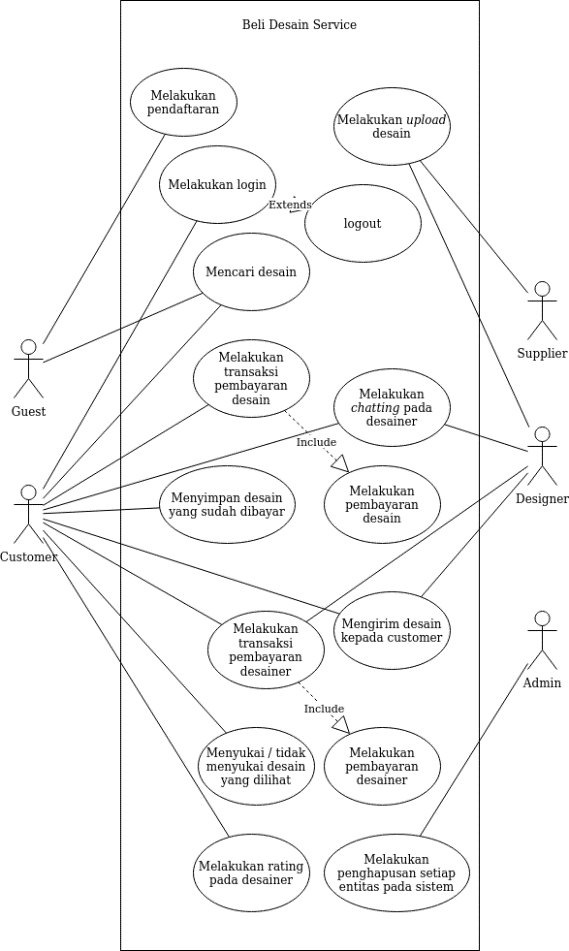
\includegraphics{usecase}
	\caption{Use Case Diagram Sistem Belidesain}
\end{figure}

\section{Identifikasi Permasalahan}
Berdasarkan latar belakang yang telah ditulis, terdapat beberapa identifikasi masalah yang dapat disimpulkan yaitu sebagai berikut:
\begin{enumerate}
	\item Penjualan desain pada platform e-commerce jarang ditemui.
	\item Penyebaran informasi pameran desain yang belum meluas.
	\item Pencarian jasa desainer panggilan masih jarang ditemui.
\end{enumerate}

\section{Identifikasi Kebutuhan Pengguna}
Semakin berkembangnya teknologi, gaya hidup masyarakat ikut serta berubah. Di era yang sekarang, gaya hidup yang diikuti masyarakat adalah gaya hidup modern. Kebutuhan masyarakat pun tidak jauh dari hal yang berkaitan dengan desain, seperti pakaian, barang perabot, dan lain-lain. Ketika akan membeli pasti mencari desain yang cocok dengan selera dan kebutuhan. Tidak jarang desain yang dicari tidak sesuai dengan selera.
\par Dalam memenuhi kebutuhan masyarakat akan desain yang sesuai selera, sistem yang kami buat dapat menjadi jawabannya. Sistem berisikan informasi terkait penjualan desain. Pelanggan dapat melihat-lihat terlebih dahulu terkait desain yang dicari. Apabila sudah menemukan yang sesuai, pelanggan dapat melakukan transaksi. Jika desain yang dicari tidak ada yang cocok, pelanggan dapat meminta desainer untuk membuatkan desain yang diinginkan. Semua hasil transaksi dan yang lainnya akan terekam dalam sistem database kami. 


\chapter{DESIGN}
\section{Conceptual Design}
\subsection{Entity Types}
	\begin{longtable}{| p{3.5cm} | p{4.0cm} | l | p{4.5cm} |}
		\hline
		Entity Name & Description & Aliases & Occurence \\
		\hline \hline
		User & Berisi tentang informasi dan status session pengguna pada website & - & Setiap user akan memiliki tiga tipe pengguna dengan tujuannya masing-masing, yaitu user, supplier, dan designer \\ \hline
		UserInfo & Berisi tentang informasi pribadi pengguna website & - & Setiap user dapat melakukan pergantian informasi sesukanya \\
		UserPhoto & Akan menjadi data untuk penyimpanan dan pengaksesan foto profil pengguna & - & Setiap user dapat melihat sekaligus melakukan pergantian foto profil \\ \hline
		UserFeedback & Menjadi wadah bagi user untuk mengirim saran atau masukan kepada developer & - & Setiap user dapat mengirim saran dan pesan lebih dari satu kali \\ \hline
		ChatSystem & Sistem chatting antara pengguna kepada supplier atau pengguna kepada designer & - & User dapat dihadapkan kepada sistem chatting saat akan/ingin melakukan pembelian desain \\ \hline
		DesignCategories & Pilihan kategori atau peminatan sebuah desain & - & Setiap kategori telah ditetapkan secara spesifik dan mendetail \\ \hline
		DesignSubCategories & Pilihan sub-kategori atau jenis desain yang dibuat berdasarkan kategori yang ada & - & Setiap sub-kategori sudah ditetapkan mengikat pada kategori/peminatan desain yang telah ada \\ \hline
		DesignTheme & Pilihan tema sebuah desain & - & Tema akan ditempatkan pada masukan user. \\ \hline
		DesignHeader & Menjadi ikatan relasi antara kategori, sub-kategori, tema, dan supplier/designer. Entitas ini berfungsi sebagai identifikasi utama dari sebuah desain dan juga status penjualan desain & - & Ikatan - ikatan relasi yang ada akan ditetapkan oleh supplier/designer \\ \hline
		DesignLikeCount & Berfungsi menampung like dan dislike masukan dari pengguna website & - & Pemilihan like dan dislike akan ditentukan oleh pengguna \\ \hline
		UserInventory & Berisi desain - desain yang telah dibeli oleh pengguna dan dapat diakses kembali. & - & Entitas ini akan muncul saat pengguna telah membeli dan melakukan transaksi desain \\ \hline
		DesignTransaction Header & Berisi status dan identifikasi transaksi antara pengguna dengan desain yang akan atau telah dibeli & - & Transaksi akan muncul jika pengguna akan membeli desain yang diinginkan \\ \hline
		DesignTransaction Details & Berisi tanggal - tanggal dan informasi penting sebuah transaksi & - & Detail transaksi akan muncul seiring transaksi diadakan \\ \hline
		DesignDetails & Berisi informasi utama tentang desain yang dijual & - & Informasi ini akan ditetapkan oleh supplier dan akan muncul seiring relasi - relasi desain diadakan \\ \hline
		DesignPhotos & Berisi pratinjau foto - foto desain yang dijual & - & Foto - foto yang diperlukan akan diupload oleh supplier/designer \\ \hline
		DesignSpesification & Berisi spesifikasi mendetail tentang desain yang dijual  & - & Spesifikasi - spesifikasi ini dapat diisi oleh pengguna \\ \hline
		DesignFile & Berisi file desain secara teknis dan runtut & - & File dapat diakses oleh pengguna jika telah membeli dan membayar transaksi jual beli desain \\ \hline
		ExpoEvent & Berisi status dan relasi penting yang berkaitan dengan penyelenggaraan event expo & - & Jadwal dan status expo akan ditetapkan oleh supplier/designer sebagai penyelenggara \\ \hline
		ExpoTransaction Header & Berisi status utama transaksi tiket untuk mengikuti expo & - & Transaksi akan dimulai saat pengguna melakukan pembelian tiket expo \\ \hline
		UserExpo & Berisi expo - expo yang telah diikuti dan dibeli tiketnya oleh pengguna & - & Expo akan muncul pada entitas ini setelah tiket dibeli oleh pengguna \\ \hline
		ExpoTransaction Details & Berisi detail tanggal - tanggal dan status penting transaksi expo berjalan & - & Detail expo akan muncul seiring dengan status utama transaksi \\ \hline
		ExpoEventDetails & Berisi informasi penyelenggaraan expo secara mendetail & - & Informasi - informasi ini akan ditulis oleh supplier/designer \\ \hline
		ExpoEventPhoto & Berisi foto - foto dan pamflet yang berisi informasi penyelenggaraan expo & - & Supplier/Designer dapat melakukan proses upload pada entitas ini \\ \hline
		DesignerTransaction Header & Berisi informasi dan relasi utama transaksi antara pengguna user dan designer & - & Transaksi akan dimulai saat pengguna user akan melakukan persewaan designer \\ \hline
		DesignerTransaction Detail & Berisi informasi tanggal dan status penting berjalannya transaksi antara user dengan designer & - & Detail informasi akan muncul saat informasi transaksi utama muncul \\ \hline
		DesignerInfo & Berisi informasi  designer & - & Informasi akan ditetapkan oleh pengguna saat pengguna user melakukan pendaftaran menjadi desainer \\ \hline
		DesignerRating & Berfungsi untuk menampung masukkan rating atau penilaian oleh user lainnya & - & Pemilihan rating akan ditetapkan oleh user yang akan melakukan penilaian \\ \hline
		\caption{Entity Types}
	\end{longtable}

\subsection{Relationship Types}
	\begin{longtable}{| p{3.4cm} | l | l | l | p{3.4cm} |}
		\hline
		Entity Name & Multiplicity & Relationship & Multiplicity & Entity Name \\
		\hline
		User & 1 & Memiliki & 1 & DesignerInfo \\ \hline
		User & 0..1 & Berkaitan & 0..* & DesignerRating \\ \hline
		User & 0..* & Berkaitan & 0..* & ChatSystem \\ \hline
		User & 1 & Memiliki & 1 & UserInfo \\ \hline
		User & 1 & Memiliki & 1 & UserPhoto \\ \hline
		User & 0..* & Berkaitan & 1..* & UserFeedback \\ \hline
		User & 0..* & Berkaitan & 1..* & DesignTransaction Header \\ \hline
		User & 0..* & Berkaitan & 1..* & DesignLikeCount \\ \hline
		User & 0..* & Berkaitan & 1..* & UserExpo \\ \hline
		User & 0..* & Berkaitan & 1..* & DesignTransaction Header \\ \hline
		User & 0..* & Memiliki & 1..* & UserInventory \\ \hline
		User & 0..* & Berkaitan & 1..* & DesignHeader \\ \hline
		User & 0..* & Berkaitan & 1..* & ExpoTransaction Header \\ \hline
		User & 0..* & Berkaitan & 1..* & ExpoEvent \\ \hline
		DesignTransaction Header & 1 & Memiliki & 1 & DesignerTransaction Details \\ \hline
		DesignTransaction Header & 1 & Memiliki & 1 & DesignTransaction Details \\ \hline
		DesignTransaction Header & 1 & Berkaitan & 1 & UserInventory \\ \hline
		DesignHeader & 1 & Berkaitan & 1 & DesignTransaction Header \\ \hline
		DesignHeader & 1 & Berkaitan & 1 & UserInventory \\ \hline
		DesignHeader & 1 & Memiliki & 1 & DesignDetails \\ \hline
		DesignHeader & 1 & Berkaitan & 0..* & DesignLikeCount \\ \hline
		ExpoTransaction Header & 1 & Memiliki & 1 & ExpoTransaction Details \\ \hline
		ExpoEvent & 1 & Berkaitan & 1 & ExpoTransaction Details \\ \hline
		ExpoEvent & 1 & Berkaitan & 1..* & ExpoTransaction Header \\ \hline
		ExpoEvent & 1 & Memiliki & 1 & ExpoEventPhoto \\ \hline
		ExpoEvent & 1 & Memiliki & 1 & ExpoEventDetails \\ \hline
		DesignDetails & 1 & Memiliki & 1 & DesignPhotos \\ \hline
		DesignDetails & 1..* & Memiliki & 1 & DesignSpesification \\ \hline
		DesignDetails & 1 & Memiliki & 1 & DesignFile \\ \hline
		DesignCategories & 1 & Berkaitan & 1 & DesignHeader \\ \hline
		DesignCategories & 1..* & Berkaitan & 1 & DesignSubCategories \\ \hline
		DesignSubCategories & 1 & Berkaitan & 1 & Design Header \\ \hline
		DesignSubCategories & 1..* & Berkaitan & 1 & DesignTheme \\ \hline
		DesignTheme & 1 & Berkaitan & 1 & DesignHeader \\ \hline
		\caption{Relationship Types}
	\end{longtable}
\subsection{Attributes}
	\begin{longtable}{| p{2.2cm} | p{2.5cm} | p{3.4cm} | p{2.2cm} | l | p{1.3cm} |}
		\hline
		Entity Name & Attribute & Description & Data Type \& Length & Nulls & Multi valued \\
		\hline
		\noindent 
		User & 	UserId			& Identifikasi User			& Int(10)		& No & No \\
			 &	Email			& Email User				& Varchar(20)	& No & No \\
			 &	Password		& Password User				& Varchar(20)	& No & No \\
			 & 	LastActivity	& Terakhir kali user Aktif	& Datetime		& No & No \\
			 &	isOnline		& User sedang Online		& Boolean		& No & No \\
			 &	isSupplier		& User seorang supplier		& Boolean		& No & No \\
			 &	isDesigner		& User seorang designer		& Boolean		& No & No \\ \hline
			 
		UserInfo 	& UserId		& Identifikasi User		& Int(10)		& No  & No \\
					& Name			& Nama User				& Varchar(50)	& No  & No \\
					& Description	& Deskripsi supplier	& Text			& Yes & Yes \\
					& Company		& Perusahaan supplier	& Varchar(48)	& Yes & Yes \\
					& Location		& Lokasi Supplier		& Varchar(48)	& Yes & Yes \\
					& Website		& Website Supplier		& Varchar(48)	& Yes & Yes \\
					& PhoneNumber	& Nomor Telp Supplier	& Varchar(16)	& Yes & Yes \\ \hline
					
		UserPhoto	& PhotoId	& Identifikasi Foto	& Int(10)		& No & No \\
					& UserId	& Identifikasi User	& Int(10)		& No & No \\
					& PhotoName	& Nama Foto			& Varchar(48)	& No & No \\ \hline
					
		UserFeed-back	& FeedbackId		& Identifikasi		& Int(10) 	& No & No \\
						& UserId			& Identifikasi User	& Int(10) 	& No & No \\
						& Feedback-Message	& Isi Masukkan User	& Text		& No & Yes \\ \hline
						
		ChatSystem	& ChatSystemId	& Identifikasi Chat		& Int(10)		& No & No \\
					& toUserId		& Identifikasi tujuan	& Int(10)		& No & No \\
					& fromUserId	& Identifikasi asal		& Int(10)		& No & No \\
					& Message		& Isi Pesan				& Varchar(100)	& No & Yes \\
					& Timestamp		& Waktu Pengiriman		& Datetime		& No & No \\
					& StatusMessage	& Konfirmasi Terkirim	& Varchar(15)	& No & No \\ \hline
					
		Design-Categories	& CategoryId	& Identifikasi kategori	& Int(10)		& No  & No \\
							& CategoryName	& Nama Kategori			& Varchar(20)	& No  & No \\
							& CategoryDesc	& Deskripsi kategori	& Text			& Yes & No \\ \hline
		
		DesignSub-Categories	& SubCategoryId		& Identifikasi subkategori	& Int(10)		& No  & No \\
							& CategoryId		& Identifikasi kategori		& Int(10)		& No  & No \\
							& SubCategory-Name	& Nama subkategori			& Varchar(64)	& No  & No \\
							& SubCategory-Desc	& Deskripsi subkategori		& Text			& Yes & No \\ \hline
							
		DesignTheme	& ThemeId		& Identifikasi tema			& Int(10)		& No & No \\
					& SubCategoryId	& Identifikasi subkategori	& Int(10)		& No & No \\
					& ThemeName		& Nama tema					& Varchar(20)	& No & No \\ \hline

		DesignHeader	& DesignId			& Identifikasi desain		& Int(10)	& No & No \\
						& CategoryId		& Identifikasi kategori		& Int(10)	& No & No \\
						& SubCategoryId		& Identifikasi subkategori	& Int(10)	& No & No \\
						& ThemeId			& Identifikasi tema			& Int(10)	& No & No \\
						& SupplierUserId	& Identifikasi supplier		& Int(10)	& No & No \\
						& isSold			& Konfirmasi supply			& Boolean	& No & No \\ \hline
		
		DesignLike-Count	& LikeCountId	& Identifikasi like		& Int(10)	& No & No \\
						& DesignId		& Identifikasi desain	& Int(10)	& No & No \\
						& UserId		& Identifikasi user		& Int(10)	& No & No \\
						& Likes			& Total like			& Int(10)	& No & No \\ \hline
		
		UserInventory	& InventoryId			& Identifikasi kepemilikan		& Int(10)	& No & No \\
						& UserId				& Identifikasi User				& Int(10)	& No & No \\
						& DesignId				& Identifikasi Desain			& Int(10)	& No & No \\
						& DesignTransac-tionId	& Identifikasi					& Int(10)	& No & No \\
						& DatePurchased			& transaksi tanggal pembelian	& Datetime	& No & No \\ \hline
						
		Design-Transaction-Header	& Design-TransactionId	& Identifikasi Transaksi	& Int(10)	& No & No \\
									& DesignId				& Identifikasi Desain		& Int(10)	& No & No \\
									& BuyerUserId			& Identifikasi User			& Int(10)	& No & No \\
									& IsSuccess				& Konfirmasi sukses			& Boolean	& No & No \\
									& IsExpired				& Konfirmasi kadaluarsa		& Boolean	& No & No \\
									& Transaction-Type		& Tipe Transaksi			& Enum		& No & No \\ \hline
									
		Design-Transaction-Details	& Design-TransactionId	& Identifikasi transaksi	& Int(10)	& No & No \\
									& Design-Transaction-Date & Tanggal transaksi			& Datetime	& No & No \\
									& ExpirationDate		& Tanggal Kadaluarsa		& Datetime	& No & No \\
									& DateCreated			& Tanggal Dibuat			& Datetime	& No & No \\ \hline
		
		Designdetails	& DesignId			& Identifikasi desain		& Int(10)		& No & No \\
						& DesignName		& Nama Desain				& Varchar(64)	& No & No \\
						& DesignDesc		& Deskripsi Desain			& Text			& No & No \\
						& DesignPrice		& Harga Desain				& Int(10)		& No & No \\
						& DesignDate-Created & Tanggal Perilisan Desain	& Datetime		& No & No \\ \hline
		
		DesignPhotos	& DesignPhotoId		& Identifikasi foto		& Int(10)		& No & No \\
						& DesignId			& Identifikasi desain	& Int(10)		& No & No \\
						& Design-PhotoName	& Nama foto				& varchar(64)	& No & No \\ \hline
						
		Design-Spesification	& SpesificationId	& Identifikasi spesifikasi	& Int(10)		& No & No \\
								& DesignId			& Identifikasi desain		& Int(10)		& No & No \\
								& Spesification-Name	& Nama Spesifikasi			& Varchar(32)	& No & No \\
								& Spesification-Desc	& Deskripsi Spesifikasi		& Varchar(32)	& No & No \\ \hline
		
		DesignFile	& DesignFileId		& Identifikasi File		& Int(10)		& No & No \\
					& DesignId			& Identifikasi desain	& Int(10)		& No & No \\ 
					& DesignFileName	& Nama file desain		& varchar(20)	& No & No \\
					& DesignFileType	& Tipe file desain		& varchar(20)	& No & No \\ \hline
		
		ExpoEvent	& ExpoEventId		& Identifikasi expo			& Int(10)	& No & No \\
					& OrganizerUserId	& Identifikasi pembuat expo	& Int(10)	& No & No \\
					& CategoryId		& Kategori Expo				& Int(10)	& No & No \\
					& DateHeld			& Tanggal dibuat			& Datetime	& No & No \\
					& IsOnline			& Tipe Expo					& Boolean	& No & No \\ \hline

		Expo-Transaction-Header	& Expo-TransactionId	& Identifikasi transaksi	& Int(10)		& No & No \\
								& ExpoEventId		& Identifikasi event		& Int(10)		& No & No \\
								& BuyerUserId		& Identifikasi pembeli		& Int(10)		& No & No \\
								& IsSuccess 		& Konfirmasi pembelian		& Boolean		& No & No \\
								& IsExpired			& Konfirmasi kadaluarsa		& Boolean		& No & No \\
								& Transaction-Type	& Jenis transaksi			& Varchar(32)	& No & No \\ \hline
		
		UserExpo	& UserId			& Identifikasi User			& Int(10)	& No & No \\
					& ExpoEventId		& Identifikasi expo			& Int(10)	& No & No \\
					& Expo-TransactionId	& Identifikasi transaksi	& Int(10)	& No & No \\
					& DatePurchased		& Tanggal Pembelian			& Datetime	& No & No \\ \hline
		
		Expo-Transaction-Details	& Expo-Transaction-Id		& Identifikasi transaksi	& Int(10)	& No & No \\
								& Expo-Transaction-Date	& Tanggal transaksi			& Datetime	& No & No \\
								& Expo-Expiration-Date	& Tanggal kadaluarsa tiket	& Datetime	& No & No \\
								& DateCreated			& Tanggal expo dibuat		& Datetime	& No & No \\ \hline
								
		Expo-Event-Details	& ExpoEventId		& Identifikasi event	& Int(10)		& No  & No \\
							& ExpoEventTitle	& Nama event			& Varchar(32)	& No  & No \\
							& ExpoEvent-Place	& Tempat Event			& Varchar(32)	& No  & Yes \\
							& ExpoEventLink		& Link Event			& Varchar(32)	& Yes & Yes \\
							& ExpoEventDesc		& Deskripsi Event		& Text			& No  & No \\
							& TicketQuota		& Kuota Event			& Int(10)		& No  & No \\
							& TicketPrice		& Harga Tiket			& Int(10)		& No  & No \\ \hline
							
		Designer-Transaction-Header	& Designer-TransactionId	& Identifikasi Transaksi	& Int(10)		& No & No \\
									& DesignerId			& Identifikasi Desainer		& Int(10)		& No & No \\
									& BuyerUserId			& Identifikasi Pembeli		& Int(10)		& No & No \\
									& IsSuccess				& Konfirmasi pembelian		& Boolean		& No & No \\
									& IsExpired				& Konfirmasi kadaluarsa		& Boolean		& No & No \\
									& Transaction-Type		& Jenis transaksi			& Varchar(32)	& No & No \\ \hline
									
		Designer-Transaction-Details	& Designer-TransactionId	& Identifikasi desainer	& Int(10)	& No & No \\
									& AssignedDate			& Tanggal mulai proyek	& Date		& No & No \\
									& DeadlineDate			& Tanggal akhir proyek	& Date		& No & No \\
									& Confirmed				& Konfirmasi proyek		& Boolean	& No & No \\ \hline
									
		DesignerInfo	& DesignerId	& Identifikasi Desainer		& Int(10)	& No & No \\
						& DesignerPrice	& Harga jasa desainer		& Int(10)	& No & No \\
						& Rating		& Total penilaian Desainer	& Int(10)	& No & No \\ \hline
						
		Designer-Rating	& RatingId		& Identifikasi Penilaian	& Int(10)	& No & No \\
						& DesignerId	& Identifikasi Desainer		& Int(10)	& No & No \\
						& UserId		& Identifikasi User			& Int(10)	& No & No \\
						& Rating		& Penilaian per user		& Int(10)	& No & No \\ \hline
		
		\caption{Attributes}
	\end{longtable}
\subsection{Attribute Domains}
List of attribute domain:
\begin{itemize}
	\item Atribut Rating pada tabel DesignerInfo adalah constraint yang bertipe integer dimana constraint ini berupa angka yang memiliki nilai minimal 1 serta maksimal 5.
	\item Atribut Rating pada tabel DesignerRating adalah constraint yang bertipe integer dimana constraint ini berupa angka yang memiliki nilai minimal 1 serta maksimal 5.
	\item Atribut PhoneNumber pada tabel UserInfo adalah constraint yang bertipe varchar dimana constraint ini memiliki panjang 13 karakter dimana karakter pertama dan kedua harus berupa angka “08” dan karakter selanjutnya berupa angka hingga mencapai 13 karakter.
	\item Atribut website pada tabel UserInfo adalah constraint yang bertipe varchar dimana constraint ini memiliki karakter berupa string yang diikuti oleh tanda titik (.), serta dilanjutkan oleh  karakter berupa string.
	\item Atribut email pada tabel User adalah constraint yang bertipe varchar dimana constraint ini memiliki karakter berupa string yang diikuti oleh tanda @, serta dilanjutkan oleh karakter berupa string lalu titik (.), dan dilanjutkan oleh karakter string.
	\item Atribut TicketQty pada tabel ExpoTransactionHeader adalah constraint yang bertipe integer dimana constraint ini berupa angka yang memiliki nilai maksimal 10.
	\item Atribut TicketQuota pada tabel ExpoEventDetails adalah constraint yang bertipe integer dimana constraint ini berupa angka yang memiliki nilai maksimal 10.
\end{itemize}

\subsection{Candidate Keys, Primary Key, and Alternate Keys}
	\begin{longtable}{| p{3cm} | p{3.2cm} | l | p{3.2cm} |}
		\hline
		Entity Name & Candidate Key & Primary Key & Alternate Key \\
		\hline
		User 						& UserId 				& UserId 				& x 					\\ \hline
		UserInfo 					& UserId 				& x 					& UserId 				\\ \hline
		UserPhoto 					& PhotoId 				& PhotoId 				& UserId 				\\
					 				& UserId				& 						&						\\ \hline
		UserFeedback				& FeedbackId			& FeedbackId			& UserId				\\
									& UserId				& 						&						\\ \hline
		ChatSystem					& ChatSystemId			& ChatSystemId			& toUserId				\\
									& toUserId				&						& fromUserId			\\
									& fromUserId			&						&						\\ \hline
		DesignCategories			& CategoryId			& CategoryId			& x						\\ \hline
		DesignSub-Categories			& SubCategoryId			& SubCategoryId			& CategoryId			\\
									& CategoryId			&						& 						\\ \hline
		DesignTheme					& ThemeId				& ThemeId				& SubCategoryId			\\
									& SubCategoryId			&						&						\\ \hline
		DesignHeader				& DesignId				& DesignId				& CategoryId			\\
									& CategoryId			&						& SubCategoryId			\\
									& SubCategoryId 		&						& ThemeId				\\
									& ThemeId				&						& SupplierUserId		\\
									& SupplierUserId		&						& 						\\ \hline
		DesignLikeCount				& LikeCountId			& LikeCountId			& DesignId				\\
									& DesignId				& 						& UserId				\\
									& UserId				& 						& 						\\ \hline
		UserInventory				& LikeCountId			& LikeCountId			& DesignId				\\
									& DesignId				& 						& UserId				\\
									& UserId				&						&						\\ \hline
		DesignTransaction-Header		& DesignTransactionId	& DesignTransactionId	& DesignId				\\
									& DesignId				&						& BuyerUserId			\\
									& BuyerUserId			&						&						\\ \hline
		DesignTransaction-Details	& Design-TransactionId	& x						& Design-TransactionId	\\ \hline
		DesignDetails				& DesignId				& x						& DesignId				\\ \hline
		DesignPhotos				& DesignPhotoId			& DesignPhotoId			& DesignId				\\
									& DesignId				&						& 						\\ \hline
		DesignSpesification			& SpesificationId		& SpesificationId		& DesignId				\\
									& DesignId				&						&						\\ \hline
		DesignFile					& DesignFileId			& DesignFileId			& DesignId				\\
									& DesignId				&						&						\\ \hline
		ExpoEvent					& ExpoEventId			& ExpoEventId			& OrganizerUserId		\\
									& OrganizerUserId		&						& CategoryId			\\
									& CategoryId			&						&						\\ \hline
		ExpoTransaction-Header		& Expo-TransactionId		& ExpoTransactionId		& ExpoEventId			\\
									& ExpoEventId			&						& BuyerUserId			\\
									& BuyerUserId			&						&						\\ \hline
		UserExpo					& UserId				& x						& UserId				\\
									& ExpoEventId			&						& ExpoEventId			\\
									& Expo-TransactionId		&						& Expo-TransactionId		\\ \hline
		ExpoTransaction-Details		& Expo-TransactionId		& x						& Expo-TransactionId		\\ \hline
		ExpoEvent-Details			& ExpoEventId			& x						& ExpoEventId			\\ \hline
		ExpoEvent-Photo				& PhotoId				& PhotoId				& ExpoEventId			\\
									& ExpoEventId			&						& 						\\ \hline
		Designer-Transaction-Header	& Designer-TransactionId	& DesignerTransactionId	& DesignerId			\\
									& DesignerId			& 						& BuyerUserId			\\
									& BuyerUserId			&						& 						\\ \hline
		Designer-Transaction-Details	& Designer-TransactionId	& x						& Designer-TransactionId	\\ \hline
		DesingerInfo				& DesignerId			& x						& DesignerId			\\ \hline
		DesignerRating				& RatingId				& RatingId				& DesignerId			\\
									& DesignerId			&						& UserId				\\
									& UserId				&						&						\\ \hline
									
		\caption{Candidate Keys, Primary Keys, dan Alternate Keys}
	\end{longtable}

\subsection{List of User Transaction}
\begin{center}
	\fbox{\begin{minipage}{17em}
			List of user transaction:
			\begin{enumerate}[A.]
				\item DesignTransactionHeader
				\item DesignTransactionDetails
				\item ExpoTransactionHeader
				\item ExpoTransactionDetails
				\item DesignerTransactionHeader
				\item DesignerTransactionDetail
			\end{enumerate}
	\end{minipage}}
\end{center}

\subsection{Entity Relationship Diagram}
\begin{figure}[h]
	\centering
	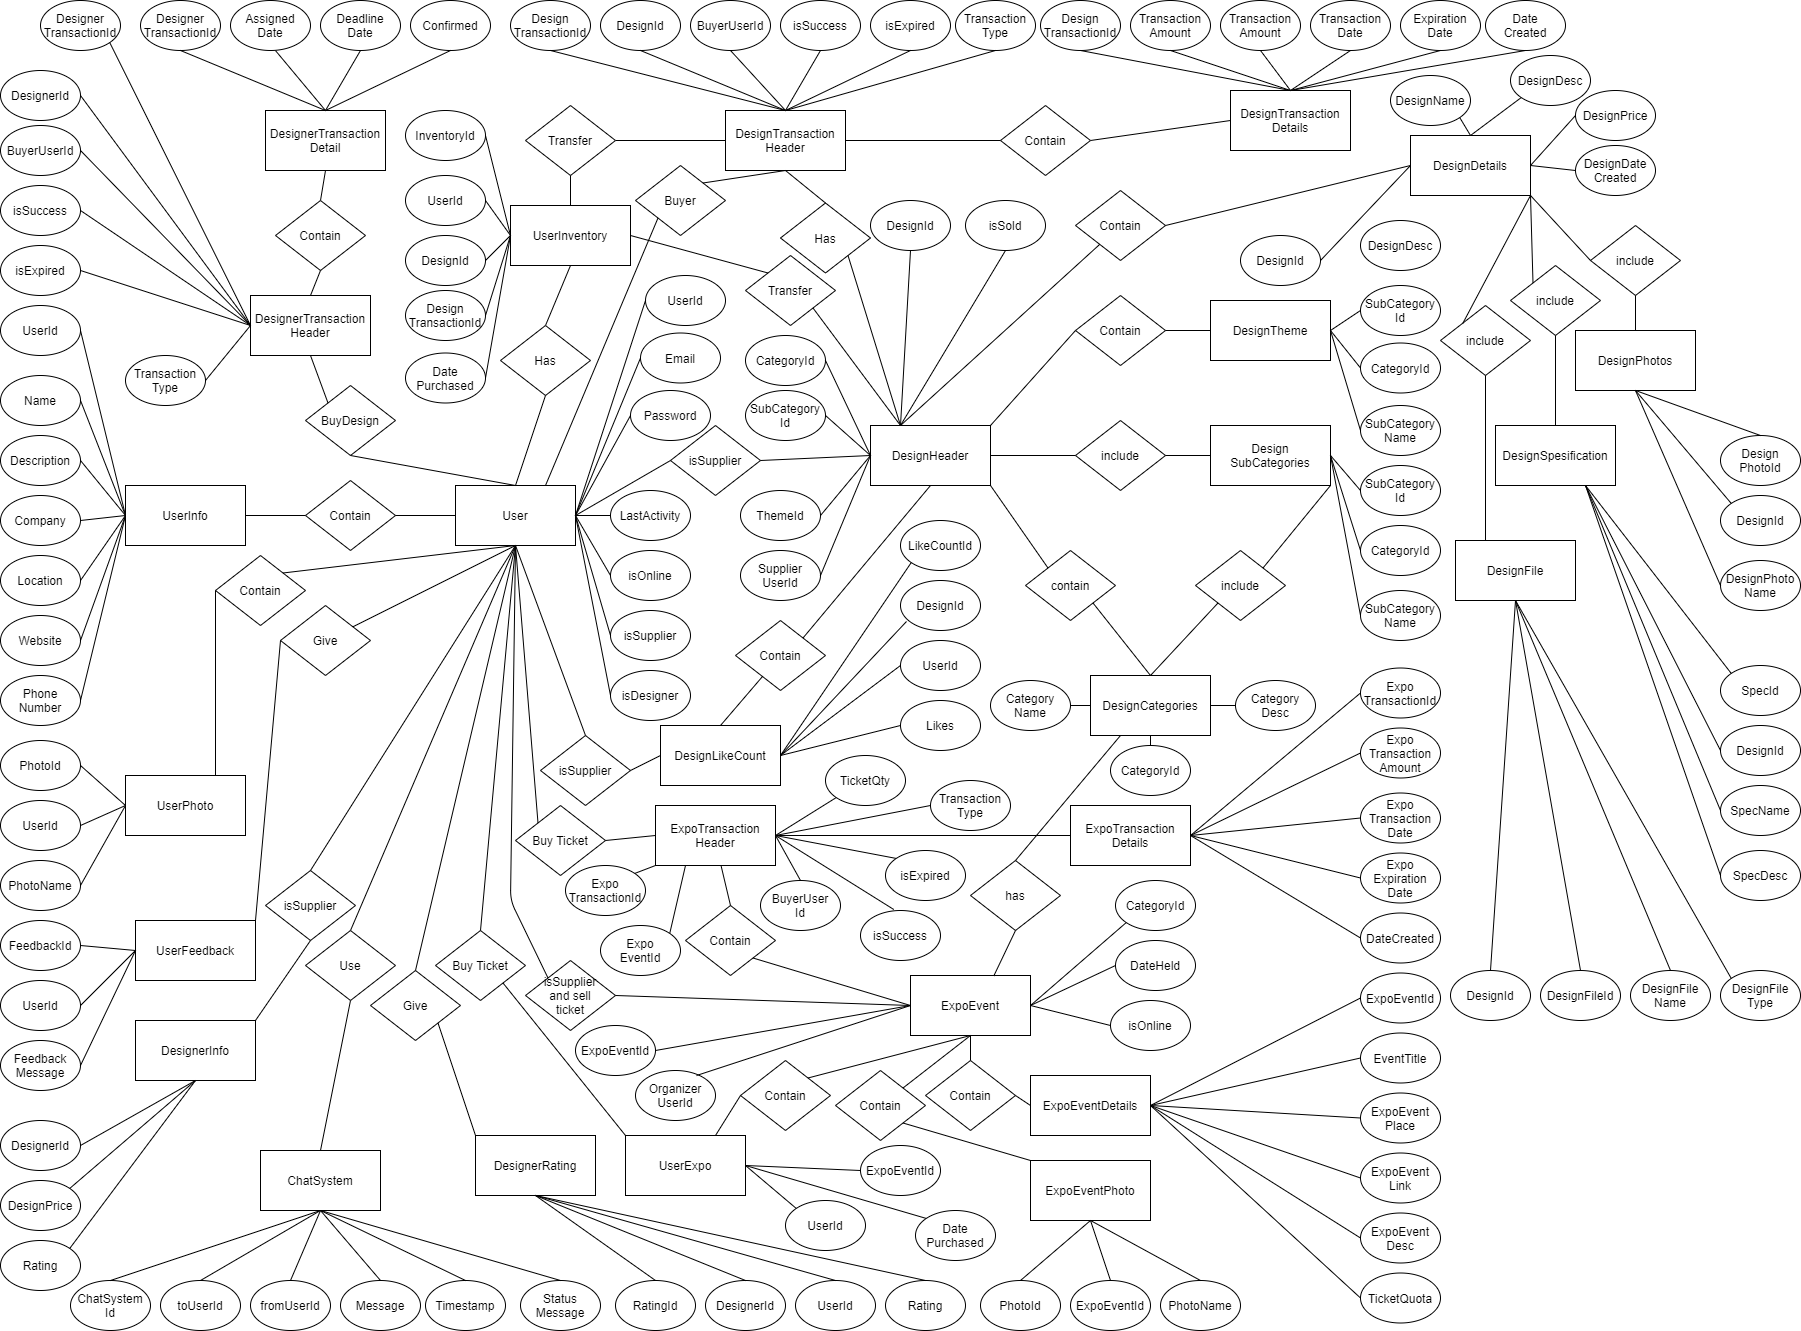
\includegraphics[width=\textwidth, height=\textheight, keepaspectratio]{erd}
	\caption{ERD Sistem Belidesain}
\end{figure}

\section{Logical Model (Class Diagram)}

\begin{figure}[H]
	\centering
	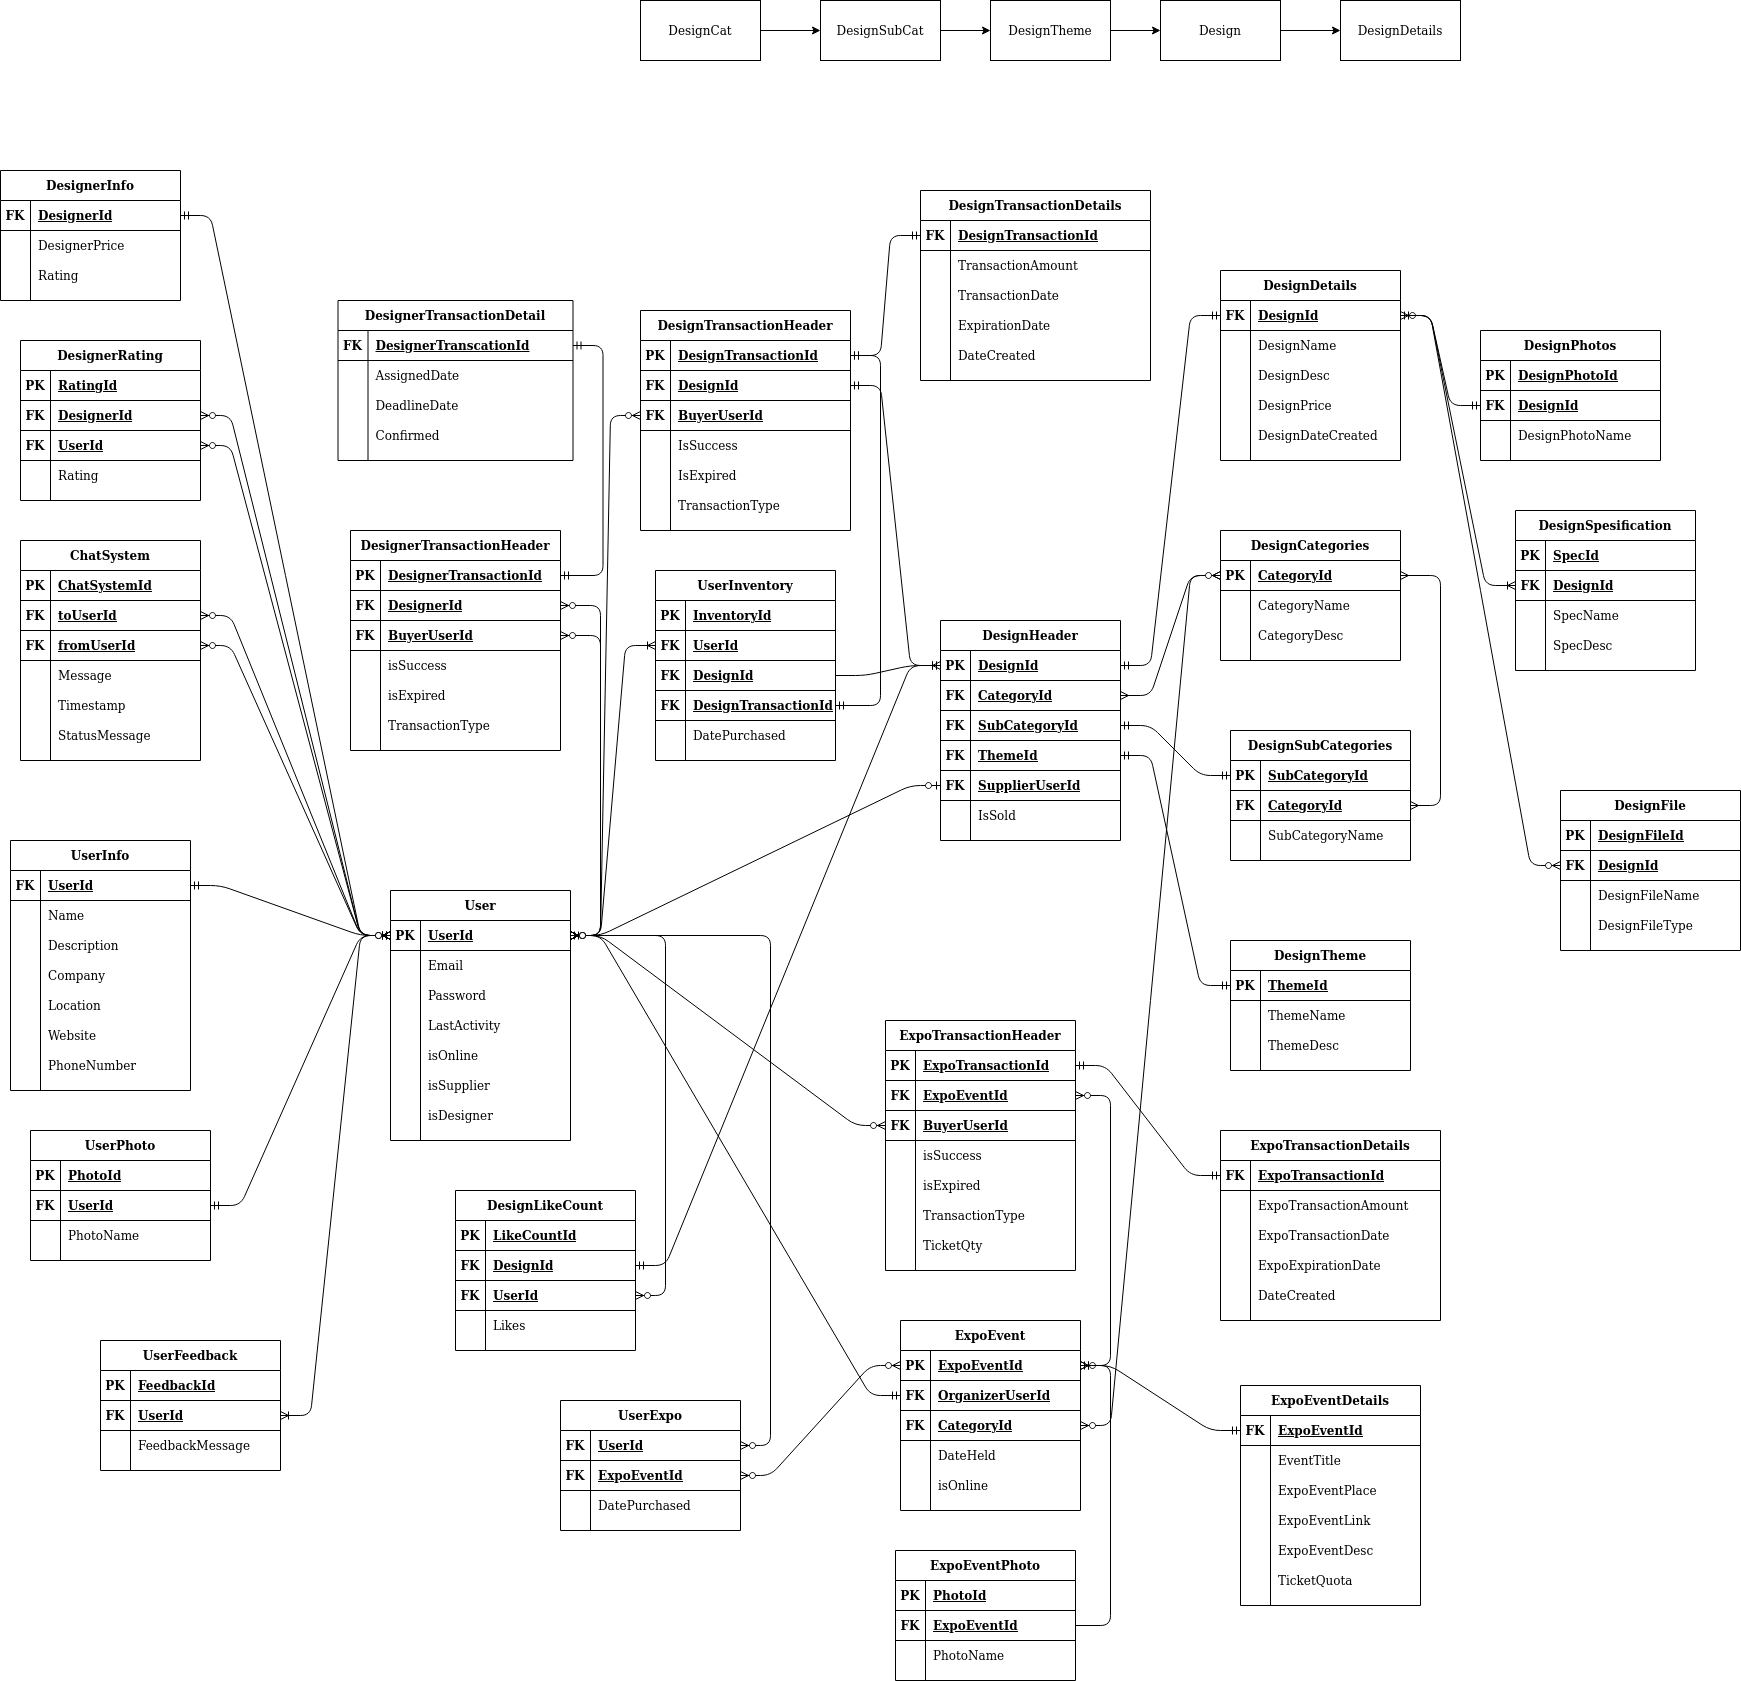
\includegraphics[width=\textwidth, height=\textheight, keepaspectratio]{classdiagram}
	\caption{Class Diagram Belidesain}
\end{figure}

\section{Physical Model}
\subsection{List of Index}
	\begin{longtable}{| p{3.0cm} | p{2.8cm} | p{3.0cm} | c | c |}
		\hline
		Entity Name 				& Index Name 			& Index 				& \multicolumn{2}{c|}{Type} \\ \cline{4-5}
									& 						&		 				& Clustered 	& Non-Clustered	\\ \hline
		User						& UserId				& UserId				& \checkmark 	& 				\\	\hline
		UserInfo					& 						&						&				& \checkmark	\\ \hline
		UserPhoto					& PhotoId				& PhotoId				& \checkmark	&				\\ \hline
		UserFeedback				& FeedbackId			& FeedbackId			& \checkmark	&				\\ \hline
		ChatSystem					& ChatSystemId			& ChatSystemId			& \checkmark	&				\\ \hline
		DesignCategories 			& CategoriesId			& CategoriesId			& \checkmark	&				\\ \hline
		DesignSub-Categories			& Sub-CategoriesId		& SubCategoriesId		& \checkmark	& 				\\ \hline
		DesignTheme					& ThemeId				& ThemeId				& \checkmark	&				\\ \hline
		DesignHeader				& DesignId				& DesignId				& \checkmark	&				\\ \hline
		DesignLikeCount				& LikeCountId			& LikeCountId			& \checkmark	& 				\\ \hline
		UserInventory				& InventoryId			& InventoryId			& \checkmark	&				\\ \hline
		DesignTransaction-Header		& Design-TransactionId	& Design-TransactionId	& \checkmark	& 				\\ \hline
		DesignTransaction-Details	& TransactionId			& TransactionId			& \checkmark	&				\\ \hline
		DesignDetails				&						&						&				& \checkmark	\\ \hline
		DesignPhotos				& DesignPhotoId			& DesignPhotoId			& \checkmark	&				\\ \hline
		DesignSpesification			& SpesificationId		& SpesificationId		& \checkmark	&				\\ \hline
		DesignFile					& DesignFileId			& DesignFileId			& \checkmark	&				\\ \hline
		ExpoEvent					& ExpoEventId			& ExpoEventId			& \checkmark	&				\\ \hline
		ExpoTransaction-Header		& ExpoTransaction-Id		& ExpoTransaction-Id		& \checkmark	&				\\ \hline
		UserExpo					& 						&						&				& \checkmark	\\ \hline
		ExpoTransaction-Header		& 						&						&				& \checkmark	\\ \hline
		ExpoEventDetails			&						&						&				& \checkmark	\\ \hline
		ExpoEventPhoto				&						&						&				& \checkmark	\\ \hline
		Designer-Transaction-Header	& Designer-TransactionId	& Designer-TransactionId	& \checkmark	&				\\ \hline
		Designer-Transaction-Details	&						&						&				& \checkmark	\\ \hline
		DesignerInfo				&						&						&				& \checkmark	\\ \hline
		DesignerRating				& RatingId				& RatingId				& \checkmark	&				\\ \hline
		\caption{List of Index}		
	\end{longtable}

\subsection{Analyze Transaction}
\definecolor{codegreen}{rgb}{0,0.6,0}
\definecolor{codegray}{rgb}{0.5,0.5,0.5}
\definecolor{codepurple}{rgb}{0.58,0,0.82}
\definecolor{backcolour}{rgb}{0.95,0.95,0.92}

\begin{table}[H]
	\centering
	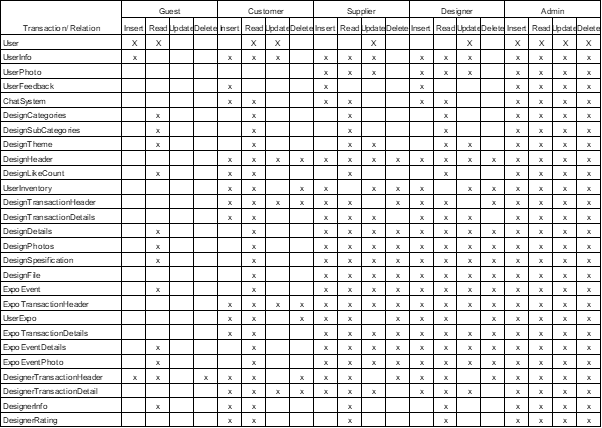
\includegraphics[width=\textwidth, height=\textheight, keepaspectratio]{analyzetransaction}
	\caption{Analyze Transaction}	
\end{table}
\subsection{User View, Procedure, and Function}
\subsubsection{Data Tabel}
\begin{table}[H]
	\centering
	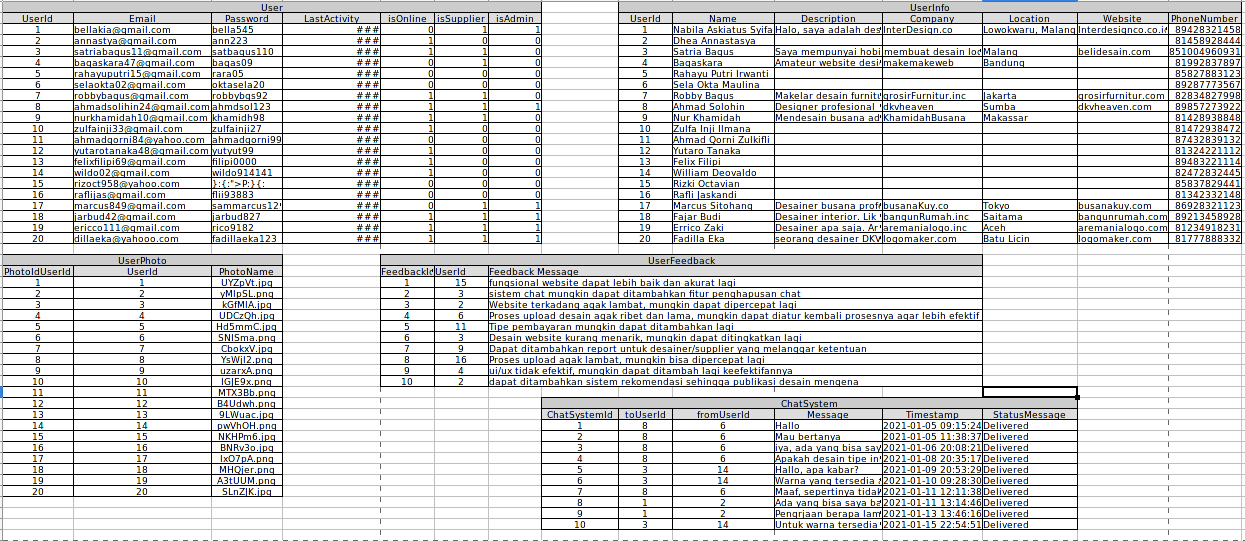
\includegraphics[width=\textwidth, height=\textheight, keepaspectratio]{insert1}
	\caption{Insert Table 1}
\end{table}
\begin{table}[H]
	\centering
	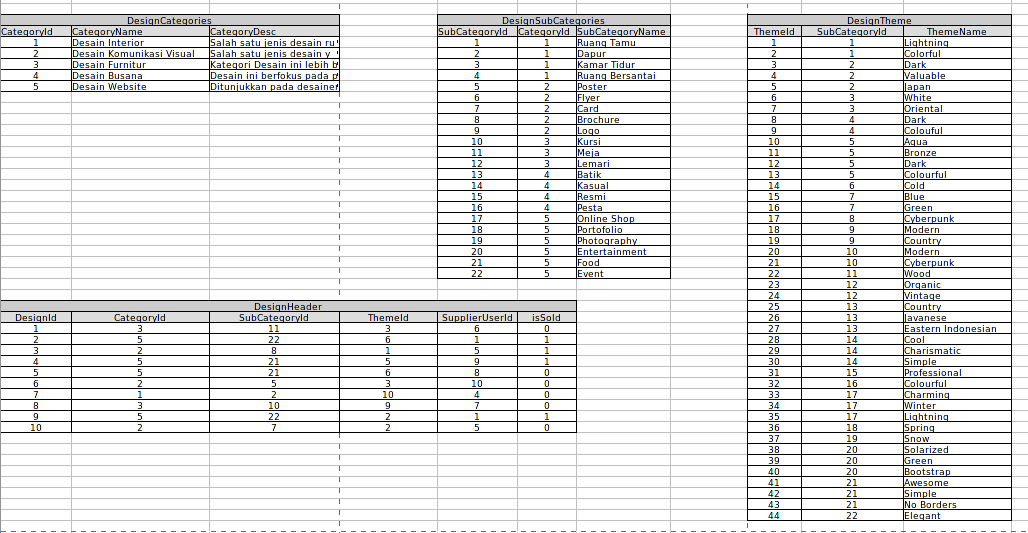
\includegraphics[width=\textwidth, height=\textheight, keepaspectratio]{insert2}
	\caption{Insert Table 2}
\end{table}
\begin{table}[H]
	\centering
	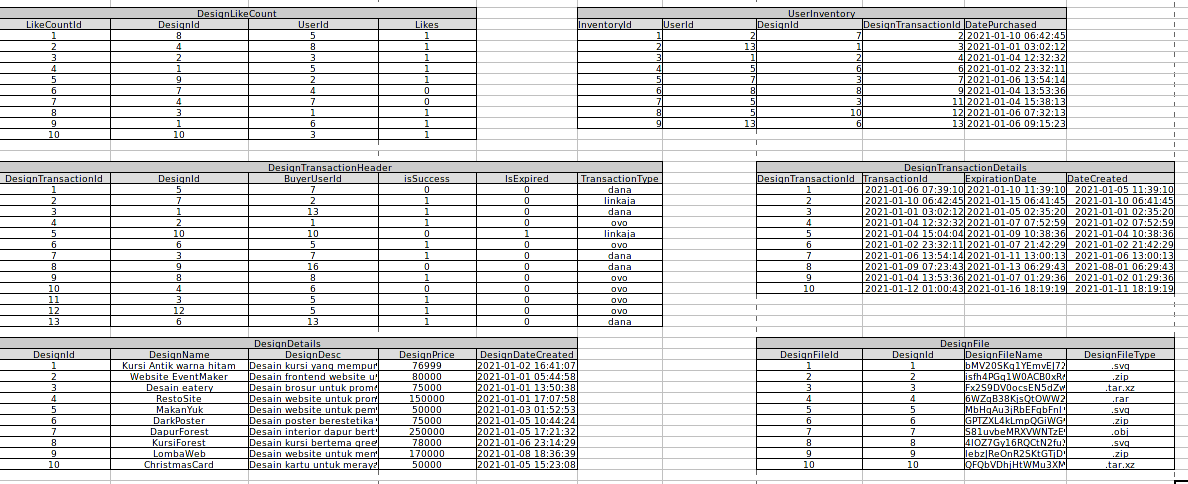
\includegraphics[width=\textwidth, height=\textheight, keepaspectratio]{insert3}
	\caption{Insert Table 3}
\end{table}
\begin{table}[H]
	\centering
	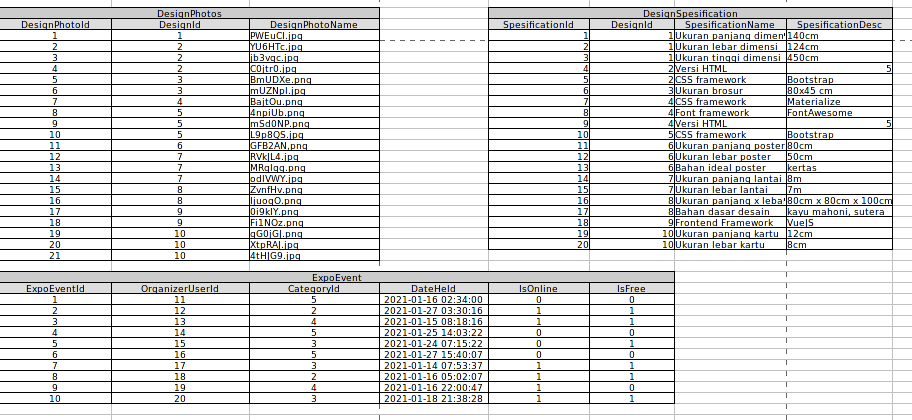
\includegraphics[width=\textwidth, height=\textheight, keepaspectratio]{insert4}
	\caption{Insert Table 4}
\end{table}
\begin{table}[H]
	\centering
	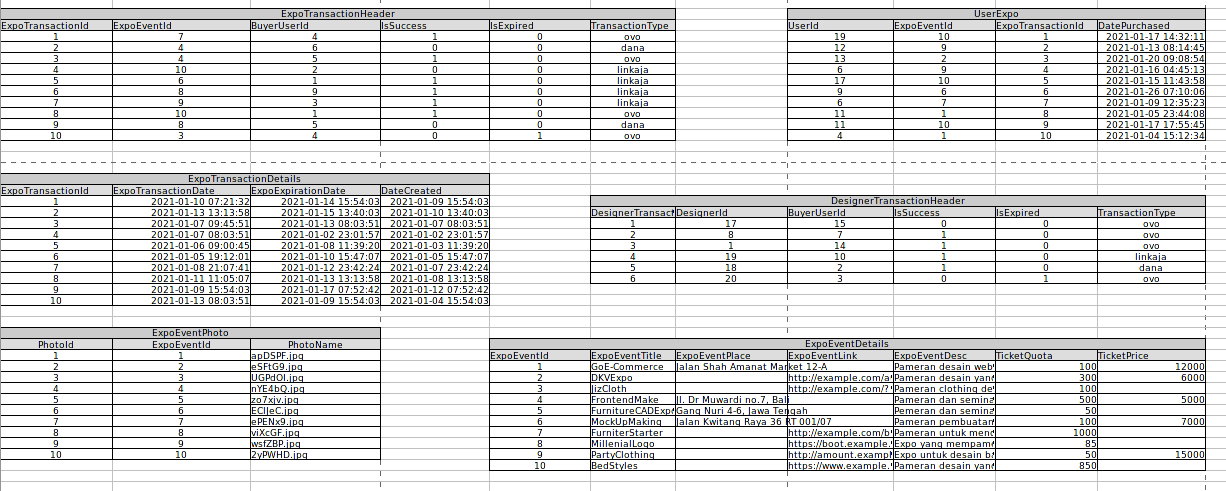
\includegraphics[width=\textwidth, height=\textheight, keepaspectratio]{insert5}
	\caption{Insert Table 5}
\end{table}
\begin{table}[H]
	\centering
	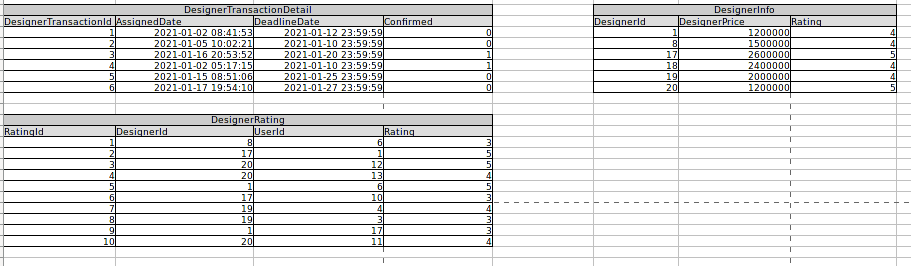
\includegraphics[width=\textwidth, height=\textheight, keepaspectratio]{insert6}
	\caption{Insert Table 6}
\end{table}
\subsubsection{User Views}
\begin{enumerate}
	\item 	Fungsi \textit{view} untuk melihat desainer dengan nilai \textit{rating} tertinggi sampai terendah \\
			Source Code :
			\begin{lstlisting}[
				language=SQL,
				backgroundcolor=\color{backcolour},   
				commentstyle=\color{codegreen},
				keywordstyle=\color{magenta},
				numberstyle=\tiny\color{codegray},
				stringstyle=\color{codepurple},
				basicstyle=\ttfamily\footnotesize,
				breakatwhitespace=false,         
				breaklines=true,                 
				captionpos=b,                    
				keepspaces=true,                 
				numbers=left,                    
				numbersep=5pt,                  
				showspaces=false,                
				showstringspaces=false,
				showtabs=false,                  
				tabsize=2]
	create view Designer_Rating_Tertinggi as
	select distinct B.Name, D.Rating
	from User A join UserInfo B
	on A.UserId = B.UserId
	join DesignerRating C
	on A.UserId = C.DesignerId
	join DesignerInfo D
	on D.DesignerId = C.DesignerId
	order by D.Rating desc;
		
	select * from Designer_Rating_Tertinggi;
	drop view Designer_Rating_Tertinggi;
			\end{lstlisting} 
		Hasil : 
		\\
		\begin{figure}[H]
			\centering
			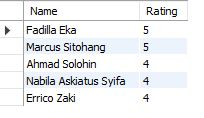
\includegraphics[width=0.4\textwidth]{view1}
			\caption{Hasil View 1}
		\end{figure}
	\item	Fungsi \textit{view} untuk melihat desain dengan harga tertinggi sampai terendah \\
			Source Code :
			\begin{lstlisting}[
				language=SQL,
				backgroundcolor=\color{backcolour},   
				commentstyle=\color{codegreen},
				keywordstyle=\color{magenta},
				numberstyle=\tiny\color{codegray},
				stringstyle=\color{codepurple},
				basicstyle=\ttfamily\footnotesize,
				breakatwhitespace=false,         
				breaklines=true,                 
				captionpos=b,                    
				keepspaces=true,                 
				numbers=left,                    
				numbersep=5pt,                  
				showspaces=false,                
				showstringspaces=false,
				showtabs=false,                  
				tabsize=2]
	create view design_harga_tertinggi as
	select B.DesignName, B.DesignPrice
	from DesignHeader A join DesignDetails B
	on A.DesignId = B.DesignId
	join User C
	on C.UserId = A.SupplierUserId
	order by B.DesignPrice desc;
	
	select * from design_harga_tertinggi;
	drop view design_harga_tertinggi;
			\end{lstlisting}
		Hasil : 
		\\
		\begin{figure}[H]
			\centering
			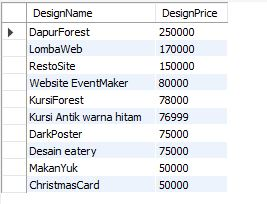
\includegraphics[width=0.4\textwidth]{view2}
			\caption{Hasil View 2}
		\end{figure}
	
	\item 	Melihat daftar transaksi dengan tipe pembayaran '\textit{ovo}' \\
			Source Code :
			\begin{lstlisting}[
				language=SQL,
				backgroundcolor=\color{backcolour},   
				commentstyle=\color{codegreen},
				keywordstyle=\color{magenta},
				numberstyle=\tiny\color{codegray},
				stringstyle=\color{codepurple},
				basicstyle=\ttfamily\footnotesize,
				breakatwhitespace=false,         
				breaklines=true,                 
				captionpos=b,                    
				keepspaces=true,                 
				numbers=left,                    
				numbersep=5pt,                  
	showspaces=false,                
	showstringspaces=false,
	showtabs=false,                  
	tabsize=2]
	create view design_harga_tertinggi as
	select B.DesignName, B.DesignPrice
	from DesignHeader A join DesignDetails B
	on A.DesignId = B.DesignId
	join User C
	on C.UserId = A.SupplierUserId
	order by B.DesignPrice desc;
	
	select * from design_harga_tertinggi;
	drop view design_harga_tertinggi;
			\end{lstlisting}
		Hasil:
		\\
		\begin{figure}[H]
			\centering
			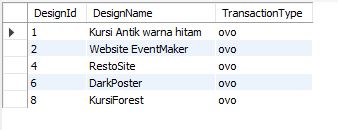
\includegraphics[width=0.6\textwidth]{view3}
			\caption{Hasil View 3}
		\end{figure}
\end{enumerate}
\subsubsection{User Triggers}
\begin{enumerate}
	\item	Fungsi \textit{trigger} untuk saat eksekusi \textit{insert}, melakukan \textit{insert} pada tabel 'UserPhoto' \\
			Source Code:
			\begin{lstlisting}[
				language=SQL,
				backgroundcolor=\color{backcolour},   
				commentstyle=\color{codegreen},
				keywordstyle=\color{magenta},
				numberstyle=\tiny\color{codegray},
				stringstyle=\color{codepurple},
				basicstyle=\ttfamily\footnotesize,
				breakatwhitespace=false,         
				breaklines=true,                 
				captionpos=b,                    
				keepspaces=true,                 
				numbers=left,                    
				numbersep=5pt,                  
				showspaces=false,                
				showstringspaces=false,
				showtabs=false,                  
				tabsize=2]
	Delimiter $$
	Create Trigger trig1
	after insert on User for each row 
	begin
	insert into UserPhoto value (NULL,new.UserId,'default.jpg');
	end $$
	Delimiter ;
	
	drop trigger trig1;
	insert into User value(NULL,'wasd@gmail.com','asd3',now(),1,0,0);
	select *from userphoto;
			\end{lstlisting}
		Hasil (Sebelum Trigger):
		\\
		\begin{figure}[H]
			\centering
			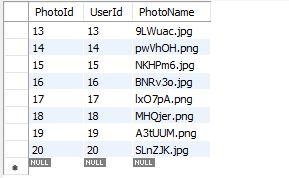
\includegraphics[width=0.6\textwidth]{trig1_before}
			\caption{Hasil Tabel Sebelum Trigger 1}
		\end{figure}
		Hasil (Setelah Trigger):
		\begin{figure}[H]
			\centering
			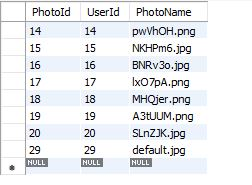
\includegraphics[width=0.6\textwidth]{trig1_after}
			\caption{Hasil Tabel Setelah Trigger 1}
		\end{figure}
	
	\item 	Fungsi \textit{trigger} untuk saat eksekusi \textit{delete}, memindahkan \textit{row} yang didelete menuju tabel \textit{temporary} \\
			Source Code:
			\begin{lstlisting}[
				language=SQL,
				backgroundcolor=\color{backcolour},   
				commentstyle=\color{codegreen},
				keywordstyle=\color{magenta},
				numberstyle=\tiny\color{codegray},
				stringstyle=\color{codepurple},
				basicstyle=\ttfamily\footnotesize,
				breakatwhitespace=false,         
				breaklines=true,                 
				captionpos=b,                    
				keepspaces=true,                 
				numbers=left,                    
				numbersep=5pt,                  
				showspaces=false,                
				showstringspaces=false,
				showtabs=false,                  
				tabsize=2]
	Delimiter $$
	Create Trigger trig2
	after delete on UserInfo for each row 
	begin
	create temporary table temp1(
	UserId INT(10) NOT NULL,
	Name VARCHAR(50) NOT NULL,
	Description TEXT,
	Company VARCHAR(48),
	Location VARCHAR(48),
	Website VARCHAR(48),
	PhoneNumber VARCHAR(16)
	);
	insert into temp1 values (old.UserId,old.name,old.description,old.company,old.location
	,old.website,old.phonenumber);
	end $$
	Delimiter ;
	
	delete from userInfo where userId=1;
			\end{lstlisting}
		Hasil (Sebelum Trigger):
		\\
		\begin{figure}[H]
			\centering
			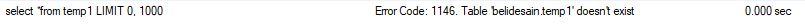
\includegraphics[width=\textwidth]{trig2_before}
			\caption{Hasil Tabel Sebelum Trigger 2}
		\end{figure}
		Hasil (Setelah Trigger):
		\begin{figure}[H]
			\centering
			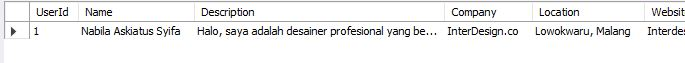
\includegraphics[width=\textwidth]{trig2_after}
			\caption{Hasil Tabel Setelah Trigger 2}
		\end{figure}
	
	\item	Fungsi \textit{trigger} untuk saat eksekusi \textit{insert}, memasukkan data kosong pada 'UserInfo' \\
			Source Code:
			\begin{lstlisting}[
				language=SQL,
				backgroundcolor=\color{backcolour},   
				commentstyle=\color{codegreen},
				keywordstyle=\color{magenta},
				numberstyle=\tiny\color{codegray},
				stringstyle=\color{codepurple},
				basicstyle=\ttfamily\footnotesize,
				breakatwhitespace=false,         
				breaklines=true,                 
				captionpos=b,                    
				keepspaces=true,                 
				numbers=left,                    
				numbersep=5pt,                  
				showspaces=false,                
				showstringspaces=false,
				showtabs=false,                  
				tabsize=2]
	Delimiter $$
	Create Trigger trig3
	after insert on User for each row 
	begin
	INSERT INTO UserInfo VALUES (new.UserId, NULL, NULL, NULL, NULL, NULL, NULL);
	end $$
	Delimiter ;
	
	insert into DesignFile value(NULL,'2','Naskle123','.svg');
			\end{lstlisting}
		Hasil (Sebelum Trigger):
		\\
		\begin{figure}[H]
			\centering
			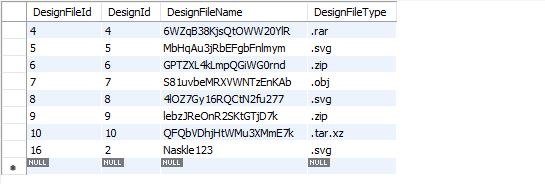
\includegraphics[width=\textwidth]{trig3_before}
			\caption{Hasil Tabel Sebelum Trigger 3}
		\end{figure}
		Hasil (Setelah Trigger):
		\begin{figure}[H]
			\centering
			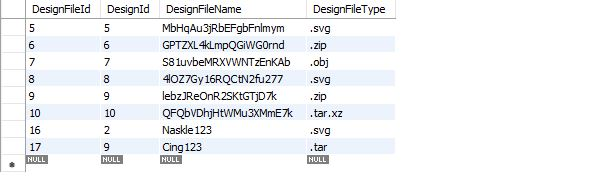
\includegraphics[width=\textwidth]{trig3_after}
			\caption{Hasil Tabel Setelah Trigger 3}
		\end{figure}
\end{enumerate}
\subsubsection{User Procedures}
\begin{enumerate}
	\item 	Fungsi \textit{Procedure} untuk melihat rata - rata \textit{rating} designer \\
	Source Code :
	\begin{lstlisting}[
		language=SQL,
		backgroundcolor=\color{backcolour},   
		commentstyle=\color{codegreen},
		keywordstyle=\color{magenta},
		numberstyle=\tiny\color{codegray},
		stringstyle=\color{codepurple},
		basicstyle=\ttfamily\footnotesize,
		breakatwhitespace=false,         
		breaklines=true,                 
		captionpos=b,                    
		keepspaces=true,                 
		numbers=left,                    
		numbersep=5pt,                  
		showspaces=false,                
		showstringspaces=false,
		showtabs=false,                  
		tabsize=2]
		Delimiter $$
		CREATE PROCEDURE getDesignerRating (
			IN DesignerId_param INT(10)
		)
		BEGIN
			SELECT 
				DesignerRating.DesignerId, 
				UserInfo.Name,
				AVG(DesignerRating.Rating) as Average
			FROM 
				DesignerRating, 
				UserInfo,User
			WHERE
				DesignerRating.DesignerId = User.UserId AND
				DesignerRating.DesignerId = DesignerId_param;
			END $$
		delimiter ;
		
		call getdesignerrating (20);
	\end{lstlisting} 
	Hasil : 
	\\
	\begin{figure}[H]
		\centering
		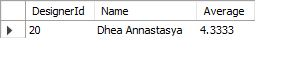
\includegraphics[width=0.4\textwidth]{proc1}
		\caption{Hasil Procedure 1}
	\end{figure}
	\item	Fungsi \textit{procedure} untuk melihat total \textit{like} pada desain \\
	Source Code :
	\begin{lstlisting}[
		language=SQL,
		backgroundcolor=\color{backcolour},   
		commentstyle=\color{codegreen},
		keywordstyle=\color{magenta},
		numberstyle=\tiny\color{codegray},
		stringstyle=\color{codepurple},
		basicstyle=\ttfamily\footnotesize,
		breakatwhitespace=false,         
		breaklines=true,                 
		captionpos=b,                    
		keepspaces=true,                 
		numbers=left,                    
		numbersep=5pt,                  
		showspaces=false,                
		showstringspaces=false,
		showtabs=false,                  
		tabsize=2]
		Delimiter $$
		CREATE PROCEDURE like_unlike(
			IN designId_param INT(10)
		)
		BEGIN
			SELECT
				DesignDetails.DesignName, 
				Count(DesignLikeCount.Likes) as 'Like'		
			FROM
				DesignHeader,
				DesignLikeCount,
				DesignDetails
			WHERE 
				DesignHeader.DesignId = DesignLikeCount.DesignId AND 
				DesignHeader.DesignId = DesignDetails.DesignId AND 
				DesignHeader.DesignId = designId_param and
				DesignLikeCount.Likes = 1;
		END $$
		delimiter ;
		
		call like_unlike (1);
	\end{lstlisting}
	Hasil : 
	\\
	\begin{figure}[H]
		\centering
		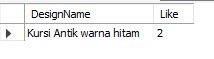
\includegraphics[width=0.4\textwidth]{proc2}
		\caption{Hasil Procedure 2}
	\end{figure}
	
	\item 	Fungsi \textit{procedure} untuk melihat total harga suatu \textit{event} \\
	Source Code:
	\begin{lstlisting}[
		language=SQL,
		backgroundcolor=\color{backcolour},   
		commentstyle=\color{codegreen},
		keywordstyle=\color{magenta},
		numberstyle=\tiny\color{codegray},
		stringstyle=\color{codepurple},
		basicstyle=\ttfamily\footnotesize,
		breakatwhitespace=false,         
		breaklines=true,                 
		captionpos=b,                    
		keepspaces=true,                 
		numbers=left,                    
		numbersep=5pt,                  
		showspaces=false,                
		showstringspaces=false,
		showtabs=false,                  
		tabsize=2]
		DELIMITER $$
		CREATE PROCEDURE total_ticket(
			IN ExpoTransactionId_param INT(10)
		)
		BEGIN
			SELECT
				ExpoEventDetails.ExpoEventTitle,
				ExpoEventDetails.TicketPrice,
				ExpoTransactionHeader.TicketQty,
				(ExpoEventDetails.TicketPrice * ExpoTransactionHeader.TicketQty) as "Total"
			FROM 
				ExpoTransactionHeader,
				ExpoEvent,
				ExpoEventDetails
			WHERE
				ExpoTransactionHeader.ExpoEventId = ExpoEvent.ExpoEventId AND
				ExpoEvent.ExpoEventId = ExpoEventDetails.ExpoEventId AND
				ExpoEvent.ExpoEventId = ExpoTransactionid_param;
			END $$
		DELIMITER ;
	\end{lstlisting}
	Hasil:
	\\
	\begin{figure}[H]
		\centering
		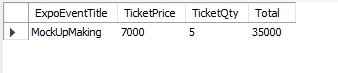
\includegraphics[width=0.6\textwidth]{proc3}
		\caption{Hasil Procedure 3}
	\end{figure}
\end{enumerate}

\chapter*{DAFTAR PUSTAKA}
\fancyhf{}
\renewcommand{\headrulewidth}{0pt}
\addcontentsline{toc}{chapter}{DAFTAR PUSTAKA}
\begin{enumerate}[label={[\arabic*]}]
	\item Irso. (2020). Dirjen PPI: Survei Penetrasi Pengguna Internet di Indonesia Bagian Penting dari Transformasi Digital. Kominfo. https://www.kominfo.go.id/content/-detail/30653/dirjen-ppi-survei-penetrasi-pengguna-internet-di-indonesia-bagian-penting-dari-transformasi-digital/0/berita\_satker
	\item Daon001. (2019). Jumlah Startup di Indonesia Ratusan atau Ribuan? Kominfo. https://kominfo.go.id/content/detail/17233/jumlah-startup-di-indonesia-ratusan-atau-ribuan/0/sorotan\_media\#:~:text=Kementerian Komunikasi dan Informatika (Kemenkominfo,itu sudah melahirkan 525 startup.
	\item “Apa itu Ecommerce? Kenali Semua Jenis dan Manfaatnya!,” Niagahoster Blog, 24-Oct-2020. [Online]. Available: https://www.niagahoster.co.id/bl-og/apa-itu-ecommerce/\#Apa\_Saja\_Jenis\_Ecommerce. [Accessed: 12-Jan-2021]. 
	\item Z. Qin et al., E-Commerce and E-Commerce Strategy. 2014.
	\item Ervina, “E-commerce : Pengertian, Jenis e commerce, dan Keuntungannya,” Talenta, 09-Nov-2020. [Online]. Available: https://www.talenta.co/blog/insight-talenta/e-commerce/\#Keuntungan\_Bisnis\_E-commerce. [Accessed: 12-Jan-2021]. 
	\item “Macam-Macam Sistem Pembayaran Pada Bisnis E-Commerce,” DAYA.ID - Inspirasi Usaha \& Kesehatan Terpercaya. [Online]. Available: https://www.daya.id/usah-a/artikel-daya/keuangan/macam-macam-sistem-pembayaran-pada-bisnis-e-commerce. [Accessed: 12-Jan-2021]. 
	\item M. Institute, “Front-End, Back-End, Full-Stack, Apa Artinya?,” Medium, 04-Apr-2017. [Online]. Available: https://medium.com/@makersinstitute/front-end-back-end-full-stack-apa-artinya-36e0f25e8142. [Accessed: 13-Jan-2021]. 
	\item "10 Skill Yang Harus Dimiliki Front End Developer - Niagahoster Blog", Niagahoster Blog, 2021. [Online]. Available: https://www.niagahoster.co.id/blog/skill-front-end-developer/\#1\_Bahasa\_Pemrograman\_HTMLCSS. [Accessed: 13- Jan- 2021].
	\item "Back End Developer: Mengenal Lingkup Kerja dan Tanggung Jawabnya", Glints Blog, 2021. [Online]. Available: https://glints.com/id/lowongan/pekerjaan-back-end-developer/\#.YAmnWegzbIV. [Accessed: 13- Jan- 2021].
	\item "12 Manfaat Basis Data dalam Kehidupan Sehari Hari - DosenIT.com", DosenIT.com, 2021. [Online]. Available: https://dosenit.com/kuliah-it/database/manfaat-basis-data. [Accessed: 21- Jan- 2021].
	\item Hidayatullah, P., \& Kawistara, J. K. (2014). Pemrograman web (Pertama). Informatika.
\end{enumerate}

\chapter*{LAMPIRAN}
\addcontentsline{toc}{chapter}{LAMPIRAN}
\fancyhf{}
\renewcommand{\headrulewidth}{0pt}
\definecolor{codegreen}{rgb}{0,0.6,0}
\definecolor{codegray}{rgb}{0.5,0.5,0.5}
\definecolor{codepurple}{rgb}{0.58,0,0.82}
\definecolor{backcolour}{rgb}{0.95,0.95,0.92}

\begin{lstlisting}[
				language=SQL,
				backgroundcolor=\color{backcolour},   
				commentstyle=\color{codegreen},
				keywordstyle=\color{magenta},
				numberstyle=\tiny\color{codegray},
				stringstyle=\color{codepurple},
				basicstyle=\ttfamily\footnotesize,
				breakatwhitespace=false,         
				breaklines=true,                 
				captionpos=b,                    
				keepspaces=true,                 
				numbers=left,                    
				numbersep=5pt,                  
				showspaces=false,                
				showstringspaces=false,
				showtabs=false,                  
				tabsize=2]
				
create database belidesain;
use belidesain;

CREATE TABLE User(
UserId INT(10) NOT NULL AUTO_INCREMENT PRIMARY KEY,
Email VARCHAR(30) NOT NULL,
Password VARCHAR(16) NOT NULL,
LastActivity DATETIME NOT NULL,
IsOnline BOOL NOT NULL,
IsSupplier BOOL NOT NULL,
IsAdmin BOOL NOT NULL,
CONSTRAINT chk_email CHECK (Email like '%@%.%')
);

CREATE TABLE UserInfo(
UserId INT(10) NOT NULL,
Name VARCHAR(50),
Description TEXT,
Company VARCHAR(48),
Location VARCHAR(48),
Website VARCHAR(48),
PhoneNumber VARCHAR(16),
FOREIGN KEY (UserId) REFERENCES User (UserId) ON DELETE CASCADE ON UPDATE CASCADE,
CONSTRAINT chk_phone CHECK (PhoneNumber regexp binary '^08[0-9][0-9][0-9][0-9][0-9][0-9][0-9][0-9][0-9][0-9]'),
CONSTRAINT chk_website CHECK (website like NULL or Website like '%.%')
);

drop table userinfo;
CREATE TABLE UserPhoto(
PhotoId  INT(10) NOT NULL AUTO_INCREMENT PRIMARY KEY,
UserId  INT(10) NOT NULL,
PhotoName VARCHAR(48) NOT NULL,
FOREIGN KEY (UserId) REFERENCES User (UserId) ON DELETE CASCADE ON UPDATE CASCADE
);

CREATE TABLE UserFeedback(
FeedbackId INT(10) NOT NULL AUTO_INCREMENT PRIMARY KEY,
UserId INT(10) NOT NULL,
FeedbackMessage TEXT NOT NULL,
FOREIGN KEY (UserId) REFERENCES User (UserId) ON DELETE CASCADE ON UPDATE CASCADE
);

CREATE TABLE ChatSystem(
ChatSystemId  INT(10) NOT NULL AUTO_INCREMENT PRIMARY KEY,
toUserId  INT(10) NOT NULL,
fromUserId  INT(10) NOT NULL,
Message VARCHAR(100) NOT NULL,
Timestamp DATETIME NOT NULL,
StatusMessage ENUM ('Pending', 'Delivered') NOT NULL,
FOREIGN KEY (toUserId) REFERENCES User (UserId) ON DELETE CASCADE ON UPDATE CASCADE,
FOREIGN KEY (fromUserId) REFERENCES User (UserId) ON DELETE CASCADE ON UPDATE CASCADE
);

CREATE TABLE DesignCategories(
CategoryId  INT(10) NOT NULL AUTO_INCREMENT PRIMARY KEY,
CategoryName VARCHAR(30) NOT NULL,
CategoryDesc TEXT NOT NULL
);

CREATE TABLE DesignSubCategories(
SubCategoryId INT(10) NOT NULL AUTO_INCREMENT PRIMARY KEY,
CategoryId INT(10) NOT NULL,
SubCategoryName VARCHAR(64) NOT NULL,
FOREIGN KEY (CategoryId) REFERENCES DesignCategories (CategoryId) ON DELETE CASCADE ON UPDATE CASCADE
);

CREATE TABLE DesignTheme(
ThemeId INT(10) NOT NULL AUTO_INCREMENT PRIMARY KEY,
SubCategoryId INT(10) NOT NULL,
ThemeName VARCHAR(20) NOT NULL,
FOREIGN KEY (SubCategoryId) REFERENCES DesignSubCategories (SubCategoryId) ON DELETE CASCADE ON UPDATE CASCADE
);

CREATE TABLE DesignHeader(
DesignId  INT(10) NOT NULL AUTO_INCREMENT PRIMARY KEY,
CategoryId  INT(10) NOT NULL,
SubCategoryId INT(10) NOT NULL,
ThemeId  INT(10) NOT NULL,
SupplierUserId INT(10) NOT NULL,
isSold BOOLEAN NOT NULL,
FOREIGN KEY (CategoryId) REFERENCES DesignCategories (CategoryId) ON DELETE CASCADE ON UPDATE CASCADE,
FOREIGN KEY (SubCategoryId) REFERENCES DesignSubCategories (SubCategoryId) ON DELETE CASCADE ON UPDATE CASCADE,
FOREIGN KEY (ThemeId) REFERENCES DesignTheme (ThemeId) ON DELETE CASCADE ON UPDATE CASCADE,
FOREIGN KEY (SupplierUserId) REFERENCES User (UserId) ON DELETE CASCADE ON UPDATE CASCADE
);

CREATE TABLE DesignLikeCount(
LikeCountId INT(10) NOT NULL AUTO_INCREMENT PRIMARY KEY,
DesignId INT(10) NOT NULL,
UserId INT(10) NOT NULL,
Likes INT(10) NOT NULL,
FOREIGN KEY (DesignId) REFERENCES DesignHeader (DesignId) ON DELETE CASCADE ON UPDATE CASCADE,
FOREIGN KEY (UserId) REFERENCES User (UserId) ON DELETE CASCADE ON UPDATE CASCADE
);

CREATE TABLE UserInventory(
InventoryId  INT(10) NOT NULL AUTO_INCREMENT PRIMARY KEY,
UserId  INT(10) NOT NULL,
DesignId  INT(10) NOT NULL,
DesignTransactionId INT(10) NOT NULL,
DatePurchased DATETIME NOT NULL,
FOREIGN KEY (UserId) REFERENCES User (UserId) ON DELETE CASCADE ON UPDATE CASCADE,
FOREIGN KEY (DesignId) REFERENCES DesignHeader (DesignId) ON DELETE CASCADE ON UPDATE CASCADE,
FOREIGN KEY (DesignTransactionId) REFERENCES DesignTransactionHeader (DesignTransactionId) ON DELETE CASCADE ON UPDATE CASCADE
);

CREATE TABLE DesignTransactionHeader(
DesignTransactionId  INT(10) NOT NULL AUTO_INCREMENT PRIMARY KEY,
DesignId INT(10) NOT NULL,
BuyerUserId INT(10) NOT NULL,
IsSuccess BOOLEAN NOT NULL,
IsExpired BOOLEAN NOT NULL,
TransactionType ENUM('ovo', 'linkaja', 'dana'),
FOREIGN KEY (DesignId) REFERENCES DesignHeader (DesignId) ON DELETE CASCADE ON UPDATE CASCADE,
FOREIGN KEY (BuyerUserId) REFERENCES User (UserId) ON DELETE CASCADE ON UPDATE CASCADE
);

CREATE TABLE DesignTransactionDetails(
DesignTransactionId  INT(10) NOT NULL,
TransactionDate DATETIME NOT NULL,
ExpirationDate DATETIME NOT NULL,
DateCreated DATETIME NOT NULL,
FOREIGN KEY (DesignTransactionId) REFERENCES DesignTransactionHeader (DesignTransactionId) ON DELETE CASCADE ON UPDATE CASCADE
);

CREATE TABLE DesignDetails(
DesignId INT(10) NOT NULL,
DesignName VARCHAR(64) NOT NULL,
DesignDesc TEXT NOT NULL,
DesignPrice INT(10) NOT NULL,
DesignDateCreated DATETIME NOT NULL,
FOREIGN KEY (DesignId) REFERENCES DesignHeader (DesignId) ON DELETE CASCADE ON UPDATE CASCADE
);

CREATE TABLE DesignPhotos(
DesignPhotoId INT(10) NOT NULL AUTO_INCREMENT PRIMARY KEY,
DesignId INT(10) NOT NULL,
DesignPhotoName VARCHAR(64) NOT NULL,
FOREIGN KEY (DesignId) REFERENCES DesignDetails (DesignId) ON DELETE CASCADE ON UPDATE CASCADE
);

CREATE TABLE DesignSpesification(
SpesificationId INT(10) NOT NULL AUTO_INCREMENT PRIMARY KEY,
DesignId INT(10) NOT NULL,
SpesificationName VARCHAR(50) NOT NULL,
SpesificationDesc VARCHAR(50) NOT NULL,
FOREIGN KEY (DesignId) REFERENCES DesignDetails (DesignId) ON DELETE CASCADE ON UPDATE CASCADE
);

CREATE TABLE DesignFile(
DesignFileId INT(10) NOT NULL AUTO_INCREMENT PRIMARY KEY,
DesignId INT(10) NOT NULL,
DesignFileName VARCHAR(20) NOT NULL,
DesignFileType VARCHAR(20) NOT NULL,
FOREIGN KEY (DesignId) REFERENCES DesignDetails (DesignId) ON DELETE CASCADE ON UPDATE CASCADE
);

CREATE TABLE ExpoEvent(
ExpoEventId INT(10) NOT NULL AUTO_INCREMENT PRIMARY KEY,
OrganizerUserId INT(10) NOT NULL,
CategoryId INT(10) NOT NULL,
DateHeld DATETIME NOT NULL,
IsOnline BOOL NOT NULL,
IsFree BOOL NOT NULL,
FOREIGN KEY (OrganizerUserId) REFERENCES User (UserId) ON DELETE CASCADE ON UPDATE CASCADE,
FOREIGN KEY (CategoryId) REFERENCES DesignCategories (CategoryId) ON DELETE CASCADE ON UPDATE CASCADE
);

CREATE TABLE ExpoTransactionHeader(
ExpoTransactionId INT(10) NOT NULL AUTO_INCREMENT PRIMARY KEY,
ExpoEventId INT(10) NOT NULL,   
BuyerUserId INT(10) NOT NULL,
IsSuccess BOOL NOT NULL,
IsExpired BOOL NOT NULL,
TransactionType ENUM('ovo','linkaja','dana') NOT NULL,
TicketQty INT(10) NOT NULL,
FOREIGN KEY (ExpoEventId) REFERENCES ExpoEvent (ExpoEventId) ON DELETE CASCADE ON UPDATE CASCADE,
FOREIGN KEY (BuyerUserId) REFERENCES User (UserId) ON DELETE CASCADE ON UPDATE CASCADE,
CONSTRAINT chk_ticketQty CHECK (TicketQty <= 10)
);

CREATE TABLE UserExpo(
UserId INT(10) NOT NULL,
ExpoEventId INT(10) NOT NULL,
ExpoTransactionId INT(10) NOT NULL,
DatePurchased DATETIME NOT NULL,
FOREIGN KEY (UserId) REFERENCES User (UserId) ON DELETE CASCADE ON UPDATE CASCADE,
FOREIGN KEY (ExpoEventId) REFERENCES ExpoEvent (ExpoEventId) ON DELETE CASCADE ON UPDATE CASCADE,
FOREIGN KEY (ExpoTransactionId) REFERENCES ExpoTransactionHeader(ExpoTransactionId) ON DELETE CASCADE ON UPDATE CASCADE
); 

CREATE TABLE ExpoTransactionDetails(
ExpoTransactionId INT(10) NOT NULL,
ExpoTransactionDate DATETIME NOT NULL,
ExpoExpirationDate DATETIME NOT NULL,
DateCreated DATETIME NOT NULL,
FOREIGN KEY (ExpoTransactionId) REFERENCES ExpoTransactionHeader (ExpoTransactionId) ON DELETE CASCADE ON UPDATE CASCADE
);

CREATE TABLE ExpoEventDetails(
ExpoEventId INT(10) NOT NULL,
ExpoEventTitle VARCHAR(50)NOT NULL,
ExpoEventPlace VARCHAR(50),
ExpoEventLink VARCHAR(50),
ExpoEventDesc TEXT NOT NULL,
TicketQuota INT(10) NOT NULL,
TicketPrice INT(10),
FOREIGN KEY (ExpoEventId) REFERENCES ExpoEvent (ExpoEventId) ON DELETE CASCADE ON UPDATE CASCADE
);

CREATE TABLE ExpoEventPhoto(
PhotoId INT(10) NOT NULL,
ExpoEventId INT(10) NOT NULL,
PhotoName VARCHAR(32) NOT NULL,
FOREIGN KEY (ExpoEventId) REFERENCES ExpoEvent (ExpoEventId) ON DELETE CASCADE ON UPDATE CASCADE
);

CREATE TABLE DesignerTransactionHeader(
DesignerTransactionId INT(10) NOT NULL AUTO_INCREMENT PRIMARY KEY,
DesignerId INT(10) NOT NULL,
BuyerUserId INT(10) NOT NULL,
IsSuccess BOOL NOT NULL,
IsExpired BOOL NOT NULL,
TransactionType ENUM('ovo', 'linkaja', 'dana') NOT NULL,
FOREIGN KEY (DesignerId) REFERENCES User (UserId) ON DELETE CASCADE ON UPDATE CASCADE,
FOREIGN KEY (BuyerUserId) REFERENCES User (UserId) ON DELETE CASCADE ON UPDATE CASCADE
);

CREATE TABLE DesignerTransactionDetail(
DesignerTransactionId INT(10) NOT NULL,
AssignedDate DATETIME NOT NULL,
DeadlineDate DATETIME NOT NULL,
Confirmed BOOL NOT NULL,
FOREIGN KEY (DesignerTransactionId) REFERENCES DesignerTransactionHeader (DesignerTransactionId) ON DELETE CASCADE ON UPDATE CASCADE
);  

CREATE TABLE DesignerInfo(
DesignerId INT(10) NOT NULL,
DesignerPrice INT(10) NOT NULL,
Rating INT(10) NOT NULL,
FOREIGN KEY (DesignerId) REFERENCES User (UserId) ON DELETE CASCADE ON UPDATE CASCADE,
CONSTRAINT chk_rating CHECK (Rating <= 5 AND Rating > 0)
);

CREATE TABLE DesignerRating(
RatingId INT(10) NOT NULL AUTO_INCREMENT PRIMARY KEY,
DesignerId INT(10) NOT NULL,
UserId INT(10) NOT NULL,
Rating INT(10) NOT NULL,
FOREIGN KEY (DesignerId) REFERENCES User (UserId) ON DELETE CASCADE ON UPDATE CASCADE,
FOREIGN KEY (UserId) REFERENCES User (UserId) ON DELETE CASCADE ON UPDATE CASCADE,
CONSTRAINT chk_rating CHECK (Rating <= 5 AND Rating > 0)
);  

/*
Categories : Desain Interior, DKV, Desain Busana, Desain Furnitur, Desain Website
SubCategories : 
----Desain Interior
|--- Ruang Tamu
|--- Dapur
|--- Kamar Tidur
|--- Ruang Bersantai
----Desain Busana
|--- Batik
|--- Kasual
|--- Resmi
|--- Pesta
----Desain Furnitur
|--- Kursi
|--- Meja
|--- Lemari
----Desain Komunikasi Visual
|--- Poster
|--- Flyer
|--- Card
|--- Brochure
----Desain Website
|--- Online Shop
|--- Portofolio
|--- Photography
|--- Entertainment
|--- Food
|--- Event
*/

INSERT INTO DesignCategories VALUES
(NULL, 'Desain Interior', 'Salah satu jenis desain rumah yang berfokus pada interior atau ruangan sebuah rumah. Disini terdapat beberapa desain berdasarkan jenis ruangan, seperti desain ruang tamu, desain kamar tidur, desain dapur, dll'),
(NULL, 'Desain Komunikasi Visual', 'Salah satu jenis desain yang bertujuan menyampaikan pesan ditambah dengan aspek visual yang bagus.'),
(NULL, 'Desain Furnitur', 'Kategori Desain ini lebih berfokus pada isi dari interior rumah, misalnya Kursi, Meja, Lemari, dll'),
(NULL, 'Desain Busana', 'Desain ini berfokus pada pakaian dan sejenisnya. Contoh kategori pada desain ini antara lain: pakaian batik, pakaian pesta, pakaian resmi, dll'),
(NULL, 'Desain Website', 'Ditunjukkan pada desainer UI/UX, desain ini lebih berfokus pada bagaiman penyajian konten pada website dibuat lebih bagus. Pada website ini terdapat banyak tema yang disajikan, misalnya online shop, entertainment, event, dll');

INSERT INTO DesignSubCategories VALUES
(NULL, '1', 'Ruang Tamu'),
(NULL, '1', 'Dapur'),
(NULL, '1', 'Kamar Tidur'),
(NULL, '1', 'Ruang Bersantai'),
(NULL, '2', 'Poster'),
(NULL, '2', 'Flyer'),
(NULL, '2', 'Card'),
(NULL, '2', 'Brochure'),
(NULL, '2', 'Logo'),
(NULL, '3', 'Kursi'),
(NULL, '3', 'Meja'),
(NULL, '3', 'Lemari'),
(NULL, '4', 'Batik'),
(NULL, '4', 'Kasual'),
(NULL, '4', 'Resmi'),
(NULL, '4', 'Pesta'),
(NULL, '5', 'Online Shop'),
(NULL, '5', 'Portofolio'),
(NULL, '5', 'Photography'),
(NULL, '5', 'Entertainment'),
(NULL, '5', 'Food'),
(NULL, '5', 'Event');



INSERT INTO User VALUES
(1, 'bellakia@gmail.com', 'bella545', '2021-01-12 19:19:49', 0, 1, 1), -- designer
(2, 'annastya@gmail.com', 'ann223', '2021-01-15 06:49:19', 1, 0, 0),
(3, 'satriabagus11@gmail.com', 'satbagus110', '2021-01-06 13:23:48', 1, 1, 0), -- suppllier
(4, 'bagaskara47@gmail.com', 'bagas09', '2021-01-10 18:40:02', 0, 1, 0), -- supplier
(5, 'rahayuputri15@gmail.com', 'rara05', '2021-01-04 08:44:42', 0, 0, 0),
(6, 'selaokta02@gmail.com', 'oktasela20', '2021-01-12 01:27:52', 0, 0, 0),
(7, 'robbybagus@gmail.com', 'robbybgs92', '2021-01-09 15:14:46', 1, 1, 0), -- supplier
(8, 'ahmadsolihin24@gmail.com', 'ahmdsol123', '2021-01-01 22:11:40', 1, 1, 1), -- designer
(9, 'nurkhamidah10@gmail.com', 'khamidh98', '2021-01-11 01:15:24', 1, 1, 0), -- supplier
(10, 'zulfainji33@gmail.com', 'zulfainji27', '2021-01-04 11:54:21', 1, 0, 0),
(11, 'ahmadqorni84@yahoo.com', 'ahmadqorni99', '2021-01-10 00:32:29', 0, 0, 0),
(12, 'yutarotanaka48@gmail.com', 'yutyut99', '2021-01-10 00:05:13', 1, 0, 0),
(13, 'felixfilipi69@gmail.com', 'filipi0000', '2021-01-02 07:07:15', 1, 0, 0),
(14, 'wildo02@gmail.com', 'wildo914141', '2021-01-13 19:42:32', 1, 0, 0),
(15, 'rizoct958@yahoo.com', '}:{:">P:}{:', '2021-01-07 02:50:33', 0, 0, 0),
(16, 'raflijas@gmail.com', 'flii93883', '2021-01-07 02:50:33', 0, 0, 0),
(17, 'marcus849@gmail.com', 'sammarcus123', '2021-01-06 22:37:20', 0, 1, 1), -- designer
(18, 'jarbud42@gmail.com', 'jarbud827', '2021-01-08 06:20:04', 1, 1, 1), -- designer
(19, 'ericco111@gmail.com', 'rico9182', '2021-01-14 13:15:01', 1, 1, 1),
(20, 'dillaeka@yahooo.com', 'fadillaeka123', '2021-01-07 09:20:50', 1, 1, 1);

INSERT INTO UserInfo VALUES
(1, 'Nabila Askiatus Syifa', 'Halo, saya adalah desainer profesional yang bertempat di daerah Malang', 'InterDesign.co', 'Lowokwaru, Malang', 'Interdesignco.co.id', '089428321458'), -- designer
(2, 'Dhea Annastasya', NULL, NULL, NULL, NULL, '081458928444'),
(3, 'Satria Bagus', 'Saya mempunyai hobi membuat desain logo. Likes coffee, Lo-fi, and Jessica Veranda', NULL, 'belidesain.com','Malang', '0851004960931'), -- supplier
(4, 'Bagaskara', 'Amateur website designer from Bandung', 'makemakeweb', 'Bandung', NULL, '081992837897'), -- supplier
(5, 'Rahayu Putri Irwanti', NULL, NULL, NULL, NULL, '085827883123'),
(6, 'Sela Okta Maulina', NULL, NULL, NULL, NULL, '089287773567'),
(7, 'Robby Bagus', 'Makelar desain furnitur di grosirfurnitur.com', 'grosirFurnitur.inc', 'grosirfurnitur.com', 'Jakarta', '082834827998'), -- supplier
(8, 'Ahmad Solohin', 'Designer profesional yang berfokus pada DKV dan Desain Website', 'dkvheaven', 'dkvheaven.com', 'Sumba', '089857273922'), -- designer
(9, 'Nur Khamidah', 'Mendesain busana adalah side job sayaaa', 'KhamidahBusana', NULL,'Makassar', '081428938848'), -- supplier
(10, 'Zulfa Inji Ilmana', NULL, NULL, NULL, NULL, '081472938472'),
(11, 'Ahmad Qorni Zulkifli', NULL, NULL, NULL, NULL, '087432839132'),
(12, 'Yutaro Tanaka', NULL, NULL, NULL, NULL, '081324221112'),
(13, 'Felix Filipi', NULL, NULL, NULL, NULL, '089483221114'),
(14, 'William Deovaldo', NULL, NULL, NULL, NULL, '082472832445'),
(15, 'Rizki Octavian', NULL, NULL, NULL, NULL, '085837829441'),
(16, 'Rafli Jaskandi', NULL, NULL, NULL, NULL, '081342332148'),
(17, 'Marcus Sitohang', 'Desainer busana profesionnal', 'busanaKuy.co', 'busanakuy.com','Tokyo', '086928321123'),
(18, 'Fajar Budi', 'Desainer interior. Likes anime, babymetal, and cute', 'bangunRumah.inc', 'bangunrumah.com','Saitama','089213458928'),
(19, 'Errico Zaki', 'Desainer apa saja. Aremania', 'aremanialogo.inc', 'aremanialogo.com','Aceh', '081234918231'),
(20, 'Fadilla Eka', 'seorang desainer DKV bertempat di Jakarta', 'logomaker.com', 'logomaker.com','Batu Licin','081777888332');


INSERT INTO UserPhoto VALUES
(1, 1, 'UYZpVt.jpg'),
(2, 2, 'yMlpSL.png'),
(3, 3, 'kGfMlA.jpg'),
(4, 4, 'UDCzQh.jpg'),
(5, 5, 'Hd5mmC.jpg'),
(6, 6, 'SNISma.png'),
(7, 7, 'CbokxV.jpg'),
(8, 8, 'YsWjl2.png'),
(9, 9, 'uzarxA.png'),
(10, 10, 'IGJE9x.png'),
(11, 11, 'MTX3Bb.png'),
(12, 12, 'B4Udwh.png'),
(13, 13, '9LWuac.jpg'),
(14, 14, 'pwVhOH.png'),
(15, 15, 'NKHPm6.jpg'),
(16, 16, 'BNRv3o.jpg'),
(17, 17, 'lxO7pA.png'),
(18, 18, 'MHQjer.png'),
(19, 19, 'A3tUUM.png'),
(20, 20, 'SLnZJK.jpg');

INSERT INTO UserFeedback VALUES
(1, 15, 'fungsional website dapat lebih baik dan akurat lagi'),
(2, 3, 'sistem chat mungkin dapat ditambahkan fitur penghapusan chat'),
(3, 2, 'Website terkadang agak lambat, mungkin dapat dipercepat lagi'),
(4, 6, 'Proses upload desain agak ribet dan lama, mungkin dapat diatur kembali prosesnya agar lebih efektif'),
(5, 11, 'Tipe pembayaran mungkin dapat ditambahkan lagi'),
(6, 3, 'Desain website kurang menarik, mungkin dapat ditingkatkan lagi'),
(7, 9, 'Dapat ditambahkan report untuk desainer/supplier yang melanggar ketentuan'),
(8, 16, 'Proses upload agak lambat, mungkin bisa dipercepat lagi'),
(9, 4, 'ui/ux tidak efektif, mungkin dapat ditambah lagi keefektifannya'),
(10, 2, 'dapat ditambahkan sistem rekomendasi sehingga publikasi desain mengena');

INSERT INTO ChatSystem VALUES
(1, 8, 6, 'Hallo','2021-01-05 09:15:24','Delivered'),
(2, 8, 6, 'Mau bertanya','2021-01-05 11:38:37','Delivered'),
(3, 8, 6, 'iya, ada yang bisa saya bantu?','2021-01-06 20:08:21','Delivered'),
(4, 8, 6, 'Apakah desain tipe ini dapat dibuat dengan bahan kayu jati?','2021-01-08 20:35:17','Delivered'),
(5, 3, 14, 'Hallo, apa kabar?','2021-01-09 20:53:29','Delivered'),
(6, 3, 14, 'Warna yang tersedia apa saja?','2021-01-10 09:28:30','Delivered'),
(7, 8, 6, 'Maaf, sepertinya tidak bisa pak','2021-01-11 12:11:38','Delivered'),
(8, 1, 2, 'Ada yang bisa saya bantu?','2021-01-11 13:14:46','Delivered'),
(9, 1, 2, 'Pengrjaan berapa lama ya?','2021-01-13 13:46:16','Delivered'),
(10, 3, 14, 'Untuk warna tersedia warna merah, biru, dan putih pak','2021-01-15 22:54:51','Delivered');

INSERT INTO DesignLikeCount VALUES
(1, 8, 5, 1),
(2, 4, 8, 1),
(3, 2, 3, 1),
(4, 1, 5, 1),
(5, 9, 2, 1),
(6, 7, 4, 0),
(7, 4, 7, 0),
(8, 3, 1, 1),
(9, 1, 6, 1),
(10, 10, 3, 1);

INSERT INTO UserInventory VALUES
(1, 2, 7, 2, '2021-01-10 06:42:45'),
(2, 13, 1, 3, '2021-01-01 03:02:12'),
(3, 1, 2, 4, '2021-01-04 12:32:32'),
(4, 5, 6, 6, '2021-01-02 23:32:11'),
(5, 7, 3, 7, '2021-01-06 13:54:14'),
(6, 8, 8, 9, '2021-01-04 13:53:36');

INSERT INTO DesignTransactionHeader VALUES
(1, 5, 7, 0, 0, 'dana'),
(2, 7, 2, 1, 0, 'linkaja'),
(3, 1, 13, 1, 0, 'ovo'),
(4, 2, 1, 1, 0, 'ovo'),
(5, 10, 10, 0, 1, 'linkaja'),
(6, 6, 5, 1, 0, 'ovo'),
(7, 3, 7, 1, 0, 'dana'),
(8, 9, 16, 0, 0, 'dana'),
(9, 8, 8, 1, 0, 'ovo'),
(10, 4, 6, 0, 0, 'ovo');

INSERT INTO DesignerTransactionHeader VALUES 
(1, 17, 15, 0, 0, 'ovo'),
(2, 8, 7, 1, 0, 'ovo'),
(3, 1, 14, 1, 0, 'ovo'),
(4, 19, 10, 1, 0, 'linkaja'),
(5, 18, 2, 1, 0, 'dana'),
(6, 20, 3, 0, 1, 'ovo');

INSERT INTO DesignerTransactionDetail VALUES
(1, '2021-01-02 08:41:53', '2021-01-12 23:59:59', 0),
(2, '2021-01-05 10:02:21', '2021-01-10 23:59:59', 0),
(3, '2021-01-16 20:53:52', '2021-01-20 23:59:59', 1),
(4, '2021-01-02 05:17:15', '2021-01-10 23:59:59', 1),
(5, '2021-01-15 08:51:06', '2021-01-25 23:59:59', 0),
(6, '2021-01-17 19:54:10', '2021-01-27 23:59:59', 0);

INSERT INTO DesignerInfo VALUES 
(1, '1200000', 4.2),
(8, '1500000', 4.3),
(17, '2600000', 4.8),
(18, '2400000', 3.6),
(19, '2000000', 4.2),
(20, '1200000', 4.5); 

INSERT INTO DesignerRating VALUES 
(1, 8, 6, 3),
(2, 17, 1, 5),
(3, 20, 12, 5),
(4, 20, 13, 4),
(5, 1, 6, 5),
(6, 17, 10, 3),
(7, 19, 4, 4),
(8, 19, 3, 3),
(9, 1, 17, 3),
(10, 20, 11, 4);

INSERT INTO UserExpo VALUES
(19, 10,1, '2021-01-17 14:32:11'),
(12, 9,2, '2021-01-13 08:14:45'),
(13, 2,3, '2021-01-20 09:08:54'),
(6, 9,4, '2021-01-16 04:45:13'),
(17, 10,5, '2021-01-15 11:43:58'),
(9, 6,6, '2021-01-26 07:10:06'),
(6, 7,7, '2021-01-09 12:35:23'),
(11, 1,8, '2021-01-05 23:44:08'),
(11, 10,9, '2021-01-17 17:55:45'),
(4, 1,10, '2021-01-04 15:12:34');

INSERT INTO DesignTransactionDetails VALUES
(1,  '2021-01-06 07:39:10', '2021-01-10 11:39:10', '2021-01-05 11:39:10'),
(2,  '2021-01-10 06:42:45', '2021-01-15 06:41:45', '2021-01-10 06:41:45'),
(3,  '2021-01-01 03:02:12', '2021-01-05 02:35:20', '2021-01-01 02:35:20'),
(4,  '2021-01-04 12:32:32', '2021-01-07 07:52:59', '2021-01-02 07:52:59'),
(5,  '2021-01-04 15:04:04', '2021-01-09 10:38:36', '2021-01-04 10:38:36'),
(6,  '2021-01-02 23:32:11', '2021-01-07 21:42:29', '2021-01-02 21:42:29'),
(7,  '2021-01-06 13:54:14', '2021-01-11 13:00:13', '2021-01-06 13:00:13'),
(8,  '2021-01-09 07:23:43', '2021-01-13 06:29:43', '2021-08-01 06:29:43'),
(9,  '2021-01-04 13:53:36', '2021-01-07 01:29:36', '2021-01-02 01:29:36'),
(10, '2021-01-12 01:00:43', '2021-01-16 18:19:19', '2021-01-11 18:19:19');

INSERT INTO DesignTheme VALUES
(1, 1, 'Lightning'),
(2, 1, 'Colorful'),
(3, 2, 'Dark'),
(4, 2, 'Valuable'),
(5, 2, 'Japan'),
(6, 3, 'White'),
(7, 3, 'Oriental'),
(8, 4, 'Dark'),
(9, 4, 'Colouful'),
(10, 5, 'Aqua'),
(11, 5, 'Bronze'),
(12, 5, 'Dark'),
(13, 5, 'Colourful'),
(14, 6, 'Cold'),
(15, 7, 'Blue'),
(16, 7, 'Green'),
(17, 8, 'Cyberpunk'),
(18, 9, 'Modern'),
(19, 9, 'Country'),
(20, 10, 'Modern'),
(21, 10, 'Cyberpunk'),
(22, 11, 'Wood'),
(23, 12, 'Organic'),
(24, 12, 'Vintage'),
(25, 13, 'Country'),
(26, 13, 'Javanese'),
(27, 13, 'Eastern Indonesian'),
(28, 14, 'Cool'),
(29, 14, 'Charismatic'),
(30, 14, 'Simple'),
(31, 15, 'Professional'),
(32, 16, 'Colourful'),
(33, 17, 'Charming'),
(34, 17, 'Winter'),
(35, 17, 'Lightning'),
(36, 18, 'Spring'),
(37, 19, 'Snow'),
(38, 20, 'Solarized'),
(39, 20, 'Green'),
(40, 20, 'Bootstrap'),
(41, 21, 'Awesome'),
(42, 21, 'Simple'),
(43, 21, 'No Borders'),
(44, 22, 'Elegant');

INSERT INTO DesignHeader VALUES
(1, 3, 11, 3, 6, 0),
(2, 5, 22, 6, 1, 1),
(3, 2, 8, 1, 5, 1),
(4, 5, 21, 5, 9, 1),
(5, 5, 21, 6, 8, 0),
(6, 2, 5, 3, 10, 0),
(7, 1, 2, 10, 4, 0),
(8, 3, 10, 9, 7, 0),
(9, 5, 22, 2, 1, 1),
(10, 2, 7, 2, 5, 0);

INSERT INTO ExpoTransactionHeader VALUES
(1, 7, 4, 1, 0, 'ovo', 1),
(2, 4, 6, 0, 0, 'dana', 3),
(3, 4, 5, 1, 0, 'ovo', 3),
(4, 10, 2, 0, 0, 'linkaja', 1),
(5, 6, 1, 1, 0, 'linkaja', 5),
(6, 8, 9, 1, 0, 'linkaja', 5),
(7, 9, 3, 1, 0, 'linkaja', 2),
(8, 10, 1, 1, 0, 'ovo', 5),
(9, 8, 5, 0, 0, 'dana', 3),
(10, 3, 4, 0, 1, 'ovo', 2);

INSERT INTO DesignDetails VALUES
(1, 'Kursi Antik warna hitam', 'Desain kursi yang mempunyai estetika antik dengan warna utama hitam. Kursi ini nyaman untuk diduduki dan tidak membuat orang capai.', 76999, '2021-01-02 16:41:07'),
(2, 'Website EventMaker', 'Desain frontend website untuk pembuatan dan publikasi event', 80000, '2021-01-01 05:44:58'),
(3, 'Desain eatery', 'Desain brosur untuk promosi makanan dan restoran', 75000, '2021-01-01 13:50:38'),
(4, 'RestoSite', 'Desain website untuk promosi makanan dan restoran', 150000, '2021-01-01 17:07:58'),
(5, 'MakanYuk', 'Desain website untuk pemesanan online kuliner', 50000, '2021-01-03 01:52:53'),
(6, 'DarkPoster', 'Desain poster berestetika hitam/dark cocok untuk konser bertema halloween', 75000, '2021-01-05 10:44:24'),
(7, 'DapurForest', 'Desain interior dapur bertema greeny dan organik, cocok untuk konsep alam liar', 250000, '2021-01-05 17:21:32'),
(8, 'KursiForest', 'Desain kursi bertema greeny dan organik, cocok untuk konsep alam liar', 78000, '2021-01-06 23:14:29'),
(9, 'LombaWeb', 'Desain website untuk mempromosikan event terutama lomba - lomba', 170000, '2021-01-08 18:36:39'),
(10, 'ChristmasCard', 'Desain kartu untuk merayakan natal dan tahun-baru', 50000, '2021-01-05 15:23:08');

INSERT INTO DesignPhotos VALUES
(1, 1, 'PWEuCI.jpg'),
(2, 2, 'YU6HTc.jpg'),
(3, 2, 'jb3vgc.jpg'),
(4, 2, 'C0jtr0.jpg'),
(5, 3, 'BmUDXe.png'),
(6, 3, 'mUZNpl.jpg'),
(7, 4, 'BajtOu.png'),
(8, 5, '4npiUb.png'),
(9, 5, 'mSd0NP.png'),
(10, 5, 'L9p8QS.jpg'),
(11, 6, 'GFB2AN,png'),
(12, 7, 'RVkJL4.jpg'),
(13, 7, 'MRqlqg.png'),
(14, 7, 'odlVWY.jpg'),
(15, 8, 'ZvnfHv.png'),
(16, 8, 'IjuoqO.png'),
(17, 9, '0i9kIY.png'),
(18, 9, 'Fi1NOz.png'),
(19, 10, 'qG0jGJ.png'),
(20, 10, 'XtpRAJ.jpg'),
(21, 10, '4tHJG9.jpg');


INSERT INTO ExpoTransactionDetails VALUES
(1, '2021-01-10 07:21:32', '2021-01-14 15:54:03', '2021-01-09 15:54:03'),
(2, '2021-01-13 13:13:58', '2021-01-15 13:40:03', '2021-01-10 13:40:03'),
(3, '2021-01-07 09:45:51', '2021-01-13 08:03:51', '2021-01-07 08:03:51'),
(4, '2021-01-07 08:03:51', '2021-01-02 23:01:57', '2021-01-02 23:01:57'),
(5, '2021-01-06 09:00:45', '2021-01-08 11:39:20', '2021-01-03 11:39:20'),
(6, '2021-01-05 19:12:01', '2021-01-10 15:47:07', '2021-01-05 15:47:07'),
(7, '2021-01-08 21:07:41', '2021-01-12 23:42:24', '2021-01-07 23:42:24'),
(8, '2021-01-11 11:05:07', '2021-01-13 13:13:58', '2021-01-08 13:13:58'),
(9,'2021-01-09 15:54:03', '2021-01-17 07:52:42', '2021-01-12 07:52:42'),
(10, '2021-01-13 08:03:51', '2021-01-09 15:54:03', '2021-01-04 15:54:03');

INSERT INTO ExpoEvent VALUES
(1, 11, 5, '2021-01-16 02:34:00', 0,0),
(2, 12, 2, '2021-01-27 03:30:16', 1,1),
(3, 13, 4, '2021-01-15 08:18:16',1,1),
(4, 14, 5, '2021-01-25 14:03:22', 0, 0),
(5, 15, 3, '2021-01-24 07:15:22', 0, 1),
(6, 16, 5, '2021-01-27 15:40:07', 0, 0),
(7, 17, 3, '2021-01-14 07:53:37', 1, 1),
(8, 18, 2, '2021-01-16 05:02:07', 1, 1),
(9, 19, 4, '2021-01-16 22:00:47', 1, 0),
(10, 20, 3, '2021-01-18 21:38:28', 1, 1);

INSERT INTO ExpoEventPhoto VALUES
(1, 1, 'apDSPF.jpg'),
(2, 2, 'eSFtG9.jpg'),
(3, 3, 'UGPdOI.jpg'),
(4, 4, 'nYE4bQ.jpg'),
(5, 5, 'zo7xjv.jpg'),
(6, 6, 'EClJeC.jpg'),
(7, 7, 'ePENx9.jpg'),
(8, 8, 'viXcGF.jpg'),
(9, 9, 'wsfZBP.jpg'),
(10, 10, '2yPWHD.jpg');

INSERT INTO ExpoEventDetails VALUES
(1, 'GoE-Commerce', 'Jalan Shah Amanat Market 12-A', NULL, 'Pameran desain website bertema e-commerce', 100, 12000),
(2, 'DKVExpo', NULL, 'http://example.com/aunt/alarm#act', 'Pameran desain yang bertajuk komunikasi visual dan promosi', 300, 6000),
(3, 'JizCloth', NULL, 'http://example.com/?alarm=alarm&bell=believe#bells', 'Pameran clothing dengan tema milenial', 100, NULL),
(4, 'FrontendMake', 'Jl. Dr Muwardi no.7, Bali', NULL, 'Pameran dan seminar tentang pembuatan frontend pada website', 500, 5000),
(5, 'FurnitureCADExpo', 'Gang Nuri 4-6, Jawa Tengah', NULL, 'Pemeran dan seminar pembuatan desain furnitur memakai CAD', 50, NULL),
(6, 'MockUpMaking', 'Jalan Kwitang Raya 36 RT 001/07', NULL, 'Pameran pembuatan tampilan mockup sebuah website', 100, 7000),
(7, 'FurniterStarter', NULL, 'http://example.com/bedroom/ants', 'Pameran untuk mengajak mahasiswa - mahasiswa desain interior melakukan startup desain', 1000, NULL),
(8, 'MillenialLogo', NULL, 'https://boot.example.edu/acoustics', 'Expo yang mempamerkan logo yang diminati orang milenial masa kini', 85, NULL),
(9, 'PartyClothing', NULL, 'http://amount.example.com/?argument=apparel', 'Expo untuk desain baju santai dan cocok untuk pesta', 50, 15000),
(10, 'BedStyles', NULL, 'https://www.example.com/boot.html#badge', 'Pameran desain yang ideal untuk pembuatan ranjang/tempat tidur', 850, NULL);

INSERT INTO DesignSpesification VALUES
(1, 1, 'Ukuran panjang dimensi', '140cm'),
(2, 1, 'Ukuran lebar dimensi', '124cm'),
(3, 1, 'Ukuran tinggi dimensi', '450cm'),
(4, 2, 'Versi HTML', '5'),
(5, 2, 'CSS framework', 'Bootstrap'),
(6, 3, 'Ukuran brosur', '80x45 cm'),
(7, 4, 'CSS framework', 'Materialize'),
(8, 4, 'Font framework', 'FontAwesome'),
(9, 4, 'Versi HTML', '5'),
(10, 5, 'CSS framework', 'Bootstrap'),
(11, 6, 'Ukuran panjang poster', '80cm'),
(12, 6, 'Ukuran lebar poster', '50cm'),
(13, 6, 'Bahan ideal poster', 'kertas'),
(14, 7, 'Ukuran panjang lantai', '8m'),
(15, 7, 'Ukuran lebar lantai', '7m'),
(16, 8, 'Ukuran panjang x lebar x tinggi dimensi', '80cm x 80cm x 100cm'),
(17, 8, 'Bahan dasar desain', 'kayu mahoni, sutera'),
(18, 9, 'Frontend Framework', 'VueJS'),
(19, 10, 'Ukuran panjang kartu', '12cm'),
(20, 10, 'Ukuran lebar kartu', '8cm');

INSERT INTO DesignFile VALUES 
(1, 1, 'bMV20SKq1YEmvEJ72S2p', '.svg'),
(2, 2, 'isfh4PGq1W0ACB0xRdIT', '.zip'),
(3, 3, 'Fx2S9DV0ocsEN5dZwygu', '.tar.xz'),
(4, 4, '6WZqB38KjsQtOWW20YlR', '.rar'),
(5, 5, 'MbHqAu3jRbEFgbFnlmym', '.svg'),
(6, 6, 'GPTZXL4kLmpQGiWG0rnd', '.zip'),
(7, 7, 'S81uvbeMRXVWNTzEnKAb', '.obj'),
(8, 8, '4lOZ7Gy16RQCtN2fu277', '.svg'),
(9, 9, 'lebzJReOnR2SKtGTjD7k', '.zip'),
(10, 10, 'QFQbVDhjHtWMu3XMmE7k', '.tar.xz');

#view1  
create view Designer_Rating_Tertinggi as
select distinct B.Name, D.Rating
from User A join UserInfo B
on A.UserId = B.UserId
join DesignerRating C
on A.UserId = C.DesignerId
join DesignerInfo D
on D.DesignerId = C.DesignerId
order by D.Rating desc;

select * from Designer_Rating_Tertinggi;
drop view Designer_Rating_Tertinggi;

#view2
create view design_harga_tertinggi as
select B.DesignName, B.DesignPrice
from DesignHeader A join DesignDetails B
on A.DesignId = B.DesignId
join User C
on C.UserId = A.SupplierUserId
order by B.DesignPrice desc;

select * from design_harga_tertinggi;
drop view design_harga_tertinggi;

#view3  
create view transaksi_desain_ovo as
select 
DesignHeader.DesignId,
DesignDetails.DesignName,
DesignTransactionHeader.TransactionType
from
DesignTransactionHeader,
DesignHeader,
DesignDetails
where
DesignTransactionHeader.DesignId = DesignHeader.DesignId and
DesignHeader.DesignId = DesignDetails.DesignId and 
DesignTransactionHeader.TransactionType = 'ovo';
select * from transaksi_desain_ovo;

#trig1
Delimiter $$
Create Trigger trig1
after insert on User for each row 
begin
insert into UserPhoto value (NULL,new.UserId,'default.jpg');
end $$
Delimiter ;

drop trigger trig1;
insert into User value(NULL,'wasd@gmail.com','asd3',now(),1,0,0);
select *from userphoto;
select *from userinfo;
#trig2
Delimiter $$
Create Trigger trig2
after delete on UserInfo for each row 
begin
create temporary table temp1(
UserId INT(10) NOT NULL,
Name VARCHAR(50) NOT NULL,
Description TEXT,
Company VARCHAR(48),
Location VARCHAR(48),
Website VARCHAR(48),
PhoneNumber VARCHAR(16)
);
insert into temp1 values (old.UserId,old.name,old.description,old.company,old.location
,old.website,old.phonenumber);
end $$
Delimiter ;

drop trigger trig2;
drop table temp1;
delete from userInfo where userId=1;
select *from temp1;getDesignerRating

#trig3
Delimiter $$
Create Trigger trig3
after insert on User for each row 
begin
INSERT INTO UserInfo VALUES (new.UserId, NULL, NULL, NULL, NULL, NULL, NULL);
end $$
Delimiter ;

drop trigger trig3;
insert into DesignFile value(NULL,'2','Naskle123','.svg');


#procedure1
Delimiter $$
CREATE PROCEDURE getDesignerRating (
IN DesignerId_param INT(10)
)
BEGIN
SELECT 
DesignerRating.DesignerId, 
UserInfo.Name,
AVG(DesignerRating.Rating) as Average
FROM 
DesignerRating, 
UserInfo,User
WHERE
DesignerRating.DesignerId = User.UserId AND
DesignerRating.DesignerId = DesignerId_param;
END $$
delimiter ;
drop procedure getdesignerrating;
call getdesignerrating (20);

#procedure2
Delimiter $$
CREATE PROCEDURE like_unlike(
IN designId_param INT(10)
)
BEGIN
SELECT
DesignDetails.DesignName, 
Count(DesignLikeCount.Likes) as 'Like'

FROM
DesignHeader,
DesignLikeCount,
DesignDetails
where 
DesignHeader.DesignId = DesignLikeCount.DesignId AND 
DesignHeader.DesignId = DesignDetails.DesignId AND 
DesignHeader.DesignId = designId_param and
DesignLikeCount.Likes = 1;
END $$
delimiter ;

drop procedure like_unlike;
call like_unlike (1);

#procedure3
Delimiter $$
CREATE PROCEDURE total_ticket(
IN ExpoTransactionId_param INT(10)
)
BEGIN
SELECT
ExpoEventDetails.ExpoEventTitle,
ExpoEventDetails.TicketPrice,
ExpoTransactionHeader.TicketQty,
(ExpoEventDetails.TicketPrice * ExpoTransactionHeader.TicketQty) as "Total"
FROM 
ExpoTransactionHeader,
ExpoEvent,
ExpoEventDetails
WHERE
ExpoTransactionHeader.ExpoEventId = ExpoEvent.ExpoEventId AND
ExpoEvent.ExpoEventId = ExpoEventDetails.ExpoEventId AND
ExpoEvent.ExpoEventId = ExpoTransactionid_param;
END $$
DELIMITER ;
\end{lstlisting}

\bgroup
\titleformat{\chapter}{\filcenter}{}{0pt}{\normalfont\Large\bfseries}  %% remove \filcenter if not needed
\titlespacing{\chapter}{0pt}{\parskip}{-\parskip}
\chapter*{LEMBAR PENILAIAN}
\addcontentsline{toc}{chapter}{LEMBAR PENILAIAN}
\thispagestyle{empty}

\begin{tikzpicture}[remember picture, overlay]
	\draw[line width = 1pt] ($(current page.north west) + (1in,-1in)$) rectangle ($(current page.south east) + (-1in,1in)$);
\end{tikzpicture}
\begin{center}
	\Large
	SISTEM MARKETPLACE DAN EO EXPO KHUSUS PARA DESIGNER INTERIOR DAN EKSTERIOR
	
	\vspace{0.8cm}
	MATA KULIAH ISYS6028 - DATABASE \\
	SYSTEMS KELAS LA20 \\
	\vspace{0.8cm}
	Semester Ganjil 2020/2021
	
	\vspace{0.9cm}
	\renewcommand{\arraystretch}{1.6}
	\small
	\begin{tabular}{| c | p{0.42cm} | p{0.42cm} | p{0.42cm} | p{0.42cm} | p{0.42cm} | p{0.42cm} | p{0.42cm} | p{0.42cm} | p{0.42cm} | p{1.5cm} |}
		\hline
		\multirow{2}{*}{\textbf{DAFTAR MAHASISWA}} & \multicolumn{3}{|c|}{\textbf{NILAI}} & \multicolumn{3}{|c|}{\textbf{BOBOT}} & \multicolumn{3}{|c|}{\textbf{KREDIT}} & \multirow{2}{*}{\parbox{1.5cm}{\textbf{TOTAL KREDIT}}}\\ \cline{2-10}
			& \hfil 1 & 2 & 3 & 1 & 2 & 3 & 1 & 2 & 3 & \\[6pt] \hline
		
		2301922581 - Umi Harum & & & & 40\% & 40\% & 20\% & & & & \\ \hline
		2301930551 - Febrian Nugroho & & & & 40\% & 40\% & 20\% & & & & \\ \hline
		2301877590 - Felix Filipi & & & & 40\% & 40\% & 20\& & & & & \\ \hline
		\multicolumn{10}{|c|}{TOTAL} & \\ \hline
	\end{tabular}
\end{center}
KETERANGAN:
\begin{itemize}
	\item Skala Penilaian : 0 sd 100
	\item Komponen \begin{enumerate}
		\item : Laporan
		\item : Produk
		\item : Presentasi
	\end{enumerate}
\end{itemize}
\vspace{1.2cm}
\begin{center}
	\textbf{Malang, …… - ……………. …….. }\\
	\vfill
	\textbf{Wina Permana Sari }\\
	\textbf{D5975}
\end{center}
\egroup

\end{document}
